% Slide 6
\begin{frame}{Why Gaussian? The Maximum Entropy Principle}
\begin{block}{Derivation from First Principles}
Given constraints, choose the \textbf{least biased} distribution:
  \end{block}

\textbf{Optimization Problem:}
\begin{align*}
\text{Maximize: } & H(P_i) = -\sum_j p_{j|i} \log p_{j|i} \\
\text{Subject to: } & \sum_j p_{j|i} = 1 \quad \text{(probability)} \\
& \sum_j p_{j|i} d_{ij}^2 = \sigma_i^2 \quad \text{(expected distance)}
\end{align*}

\textbf{Lagrangian Solution:}
$$\mathcal{L} = H(P_i) + \lambda\left(\sum_j p_{j|i} - 1\right) + \mu\left(\sum_j p_{j|i}d_{ij}^2 - \sigma_i^2\right)$$
  
  \begin{center}
% This is CORRECT
\colorbox{yellow!30}{\parbox{\textwidth}{Result: $p_{j|i} \propto \exp(-d_{ij}^2/2\sigma_i^2)$ emerges naturally!}}
\end{center}
\end{frame}

% Slide 7
\begin{frame}{Perplexity: The Effective Number of Neighbors}
\begin{columns}
\column{0.5\textwidth}
\begin{center}
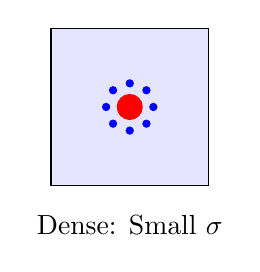
\begin{tikzpicture}[scale=1]
\draw[fill=blue!10] (-1,-1) rectangle (1,1);
\node[circle, fill=red] (center1) at (0,0) {};
\foreach \angle in {0,45,...,315} {
  \fill[blue] (\angle:0.3) circle (1.5pt);
}
\node at (0,-1.5) {Dense: Small $\sigma$};
\end{tikzpicture}
\end{center}

\column{0.5\textwidth}
\begin{center}
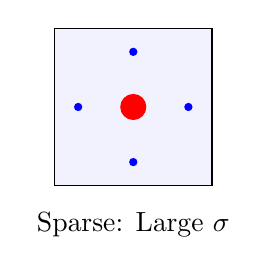
\begin{tikzpicture}[scale=1]
\draw[fill=blue!5] (-1,-1) rectangle (1,1);
\node[circle, fill=red] (center2) at (0,0) {};
\foreach \angle in {0,90,180,270} {
  \fill[blue] (\angle:0.7) circle (1.5pt);
}
\node at (0,-1.5) {Sparse: Large $\sigma$};
\end{tikzpicture}
\end{center}
\end{columns}

\vspace{0.5cm}
\begin{block}{Perplexity Definition}
$$\text{Perp}(P_i) = 2^{H(P_i)} \approx \text{effective number of neighbors}$$
  Binary search finds $\sigma_i$ to match target perplexity
\end{block}
\end{frame}

% Slide 8
\begin{frame}{Measuring Information Loss: KL Divergence}
\begin{columns}
\column{0.6\textwidth}
\begin{block}{KL Divergence}
$$\text{KL}(P||Q) = \sum_j p_j \log\frac{p_j}{q_j}$$
  Extra bits needed when using $Q$ instead of $P$
  \end{block}

\textbf{Critical Asymmetry:}
\begin{itemize}
\item \textcolor{red}{Missing a neighbor:} $p=0.3, q=0.01$
  \begin{itemize}
\item Penalty: $0.3 \log(30) \approx 1.02$ bits
\end{itemize}
\item \textcolor{blue}{False neighbor:} $p=0.01, q=0.3$
  \begin{itemize}
\item Penalty: $0.01 \log(0.033) \approx -0.035$ bits
\end{itemize}
\end{itemize}

\column{0.4\textwidth}
\begin{center}
\begin{tikzpicture}[scale=0.7]
\begin{axis}[
  ybar,
  width=6cm,
  height=5cm,
  ylabel={Probability},
  symbolic x coords={A,B,C,D},
  xtick=data,
  legend pos=north east
]
\addplot[fill=highDcolor] coordinates {(A,0.4) (B,0.3) (C,0.2) (D,0.1)};
\addplot[fill=lowDcolor] coordinates {(A,0.35) (B,0.05) (C,0.4) (D,0.2)};
\legend{$P$ (truth), $Q$ (embedding)}
\end{axis}
\end{tikzpicture}
\end{center}
\end{columns}

\vspace{0.3cm}
\insight{t-SNE heavily penalizes separating true neighbors}
\end{frame}

% Slide 9
\begin{frame}{Original SNE Algorithm}
\begin{columns}
\column{0.5\textwidth}
\textbf{High-D Similarities:}
$$p_{j|i} = \frac{\exp(-\|x_i-x_j\|^2/2\sigma_i^2)}{\sum_{k \neq i}\exp(-\|x_i-x_k\|^2/2\sigma_i^2)}$$
  
  \textbf{Low-D Similarities:}
$$q_{j|i} = \frac{\exp(-\|y_i-y_j\|^2)}{\sum_{k \neq i}\exp(-\|y_i-y_k\|^2)}$$
  
  \column{0.5\textwidth}
\textbf{Cost Function:}
$$C = \sum_i \text{KL}(P_i||Q_i)$$
  
  \textbf{Gradient:}
$$\frac{\partial C}{\partial y_i} = 2\sum_j (p_{j|i} - q_{j|i} + p_{i|j} - q_{i|j})(y_i - y_j)$$
  \end{columns}

\vspace{0.3cm}
\warning{Fatal flaw: The Crowding Problem!}
\end{frame}

% Slide 10
\begin{frame}{The Curse: Volume Distribution in High-D}
\begin{center}
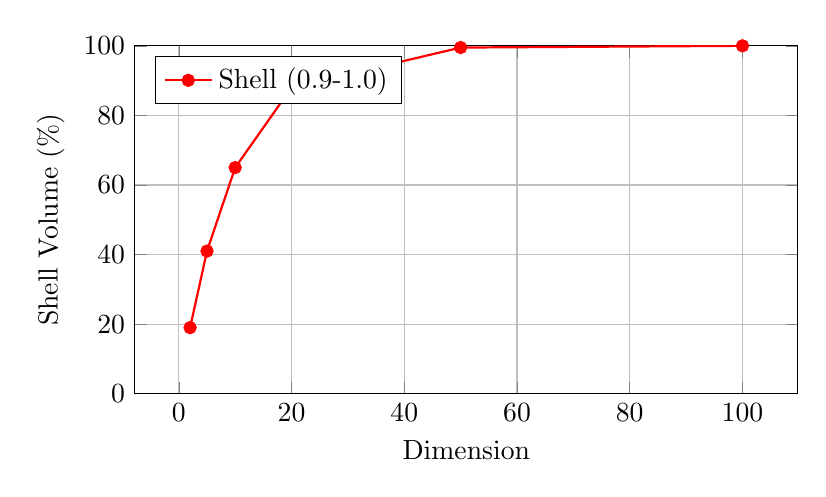
\begin{tikzpicture}
\begin{axis}[
  xlabel={Dimension},
  ylabel={Shell Volume (\%)},
  width=10cm,
  height=6cm,
  grid=major,
  ymin=0, ymax=100,
  legend pos=north west
]
\addplot[mark=*, thick, red] coordinates {
  (2,19) (5,41) (10,65) (20,88) (50,99.5) (100,99.997)
};
\addlegendentry{Shell (0.9-1.0)}
\end{axis}
\end{tikzpicture}
\end{center}

\insight{In 100D, 99.997\% of volume is in outer shell!}
\end{frame}

% ============================================
  % SLIDES 11-20: t-SNE Innovation & Core Algorithm
% ============================================
  
  % Slide 11
\begin{frame}{SNE's Fatal Flaw Visualized}
\begin{columns}
\column{0.5\textwidth}
\begin{center}
\textbf{High-D: Room for all}\\[0.3cm]
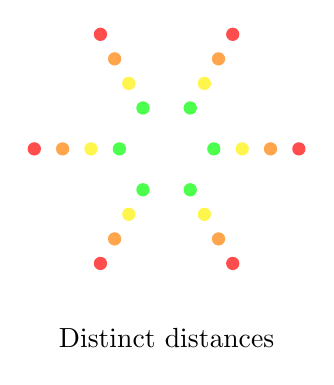
\begin{tikzpicture}[scale=1.2]
\foreach \r/\c in {0.5/green, 0.8/yellow, 1.1/orange, 1.4/red} {
    \foreach \a in {0,60,...,300} {
        \fill[\c!70] (\a:\r) circle (2pt);
    }
}
\node at (0,-2) {Distinct distances};
\end{tikzpicture}
\end{center}

\column{0.5\textwidth}
\begin{center}
\textbf{2D with Gaussian: Crushed!}\\[0.3cm]
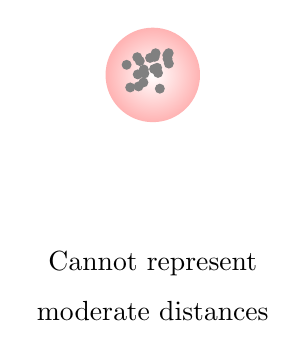
\begin{tikzpicture}[scale=1.2]
\shade[inner color=white, outer color=red!30] (0,0) circle (0.5);
\foreach \i in {1,...,20} {
    \pgfmathsetmacro\r{0.3*rnd}
    \pgfmathsetmacro\a{360*rnd}
    \fill[black!50] (\a:\r) circle (1.5pt);
}
\node at (0,-2) {Cannot represent};
\node at (0,-2.5) {moderate distances};
\end{tikzpicture}
\end{center}
\end{columns}

\vspace{0.3cm}
\begin{center}
\Large\textbf{Solution: Use distribution with heavier tails!}
\end{center}
\end{frame}

% Slide 12
\begin{frame}{The t-SNE Innovation: Student-t Distribution}
\begin{columns}
\column{0.6\textwidth}
\begin{center}
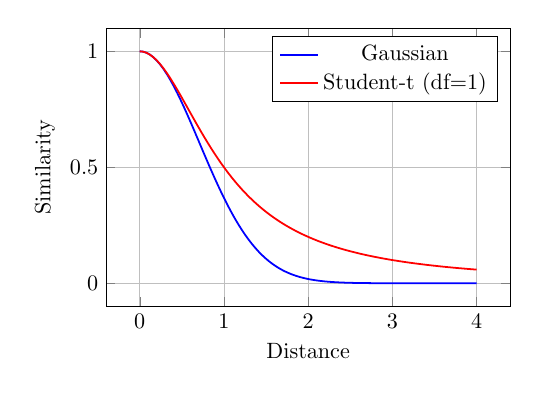
\begin{tikzpicture}[scale=0.8]
\begin{axis}[
    xlabel={Distance},
    ylabel={Similarity},
    width=8cm,
    height=6cm,
    grid=major,
    legend pos=north east,
    domain=0:4
]
\addplot[samples=100, thick, blue] {exp(-x^2)};
\addlegendentry{Gaussian}
\addplot[samples=100, thick, red] {1/(1+x^2)};
\addlegendentry{Student-t (df=1)}
\end{axis}
\end{tikzpicture}
\end{center}

\column{0.4\textwidth}
\textbf{Key Properties:}
\begin{itemize}
\item Polynomial decay
\item Heavy tails
\item More "room" at moderate distances
\end{itemize}

\vspace{0.5cm}
\insight{Creates virtual space that doesn't exist geometrically}
\end{columns}
\end{frame}

% Slide 13
\begin{frame}{Quantifying the Solution}
\begin{block}{Similarity Ratio Analysis}
For distances $d_1 = 1$ and $d_2 = 3$:
  \end{block}

\begin{columns}
\column{0.5\textwidth}
\textbf{Gaussian:}
$$\frac{q(d_1)}{q(d_2)} = \frac{e^{-1}}{e^{-9}} = e^8 \approx 2981$$
  \textcolor{red}{Moderate distance becomes "infinite"}

\column{0.5\textwidth}
\textbf{Student-t:}
$$\frac{q(d_1)}{q(d_2)} = \frac{1/(1+1)}{1/(1+9)} = 5$$
  \textcolor{green}{Moderate distance preserved}
\end{columns}

\vspace{0.5cm}
\begin{center}
\colorbox{yellow!30}{\Large 600× difference in representation capacity!}
\end{center}
\end{frame}

% Slide 14
\begin{frame}{The Complete t-SNE Algorithm}
\begin{block}{Key Modifications from SNE}
\begin{enumerate}
\item \textbf{Symmetrized:} $p_{ij} = \frac{p_{j|i} + p_{i|j}}{2n}$
  \item \textbf{Student-t in low-D:} $q_{ij} = \frac{(1+\|y_i-y_j\|^2)^{-1}}{\sum_{k \neq l}(1+\|y_k-y_l\|^2)^{-1}}$
  \item \textbf{Single KL:} $C = \text{KL}(P||Q)$ not $\sum_i \text{KL}(P_i||Q_i)$
  \end{enumerate}
\end{block}

\textbf{Cost Function:}
$$C = \sum_{i,j} p_{ij} \log\frac{p_{ij}}{q_{ij}}$$
  
  \textbf{The Elegant Gradient:}
$$\frac{\partial C}{\partial y_i} = 4\sum_j (p_{ij} - q_{ij})(y_i - y_j)(1 + \|y_i - y_j\|^2)^{-1}$$
  \end{frame}

% Slide 15
\begin{frame}{Understanding the Gradient: Force Interpretation}
\begin{center}
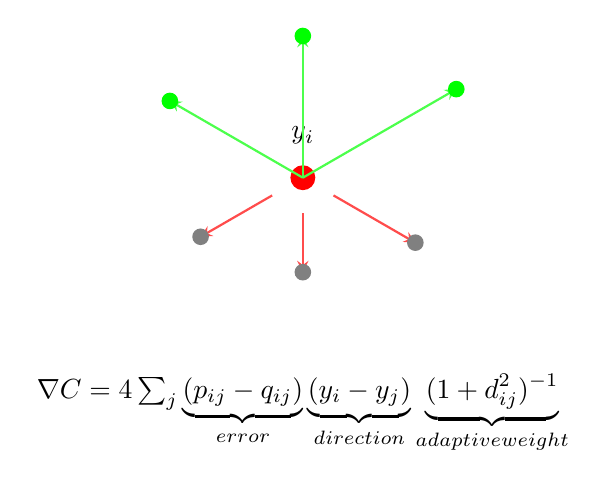
\begin{tikzpicture}[scale=1.5]
\fill[red] (0,0) circle (3pt);
\node[above] at (0,0.2) {$y_i$};

\foreach \angle/\dist in {30/1.5, 90/1.2, 150/1.3} {
  \draw[->, thick, green!70, >=stealth] (0,0) -- (\angle:\dist);
  \fill[green] (\angle:\dist) circle (2pt);
}

\foreach \angle/\dist in {210/1, 270/0.8, 330/1.1} {
  \draw[<-, thick, red!70, >=stealth] (\angle:\dist) -- (\angle:0.3);
  \fill[gray] (\angle:\dist) circle (2pt);
}

\node at (0,-2) {$\nabla C = 4\sum_j \underbrace{(p_{ij} - q_{ij})}_{\text{error}} \underbrace{(y_i - y_j)}_{\text{direction}} \underbrace{(1 + d_{ij}^2)^{-1}}_{\text{adaptive weight}}$};
\end{tikzpicture}
\end{center}

\insight{Weight term prevents distant clusters from merging}
\end{frame}

% Slide 16
\begin{frame}{Optimization Tricks for Convergence}
\begin{columns}
\column{0.33\textwidth}
\textbf{Early Exaggeration}\\[0.2cm]
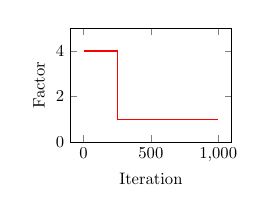
\begin{tikzpicture}[scale=0.6]
\begin{axis}[
  width=5cm,
  height=4cm,
  xlabel={Iteration},
  ylabel={Factor},
  ymin=0, ymax=5
]
\addplot[thick, red, const plot] coordinates {(0,4) (250,4) (250,1) (1000,1)};
\end{axis}
\end{tikzpicture}
Multiply $P$ by 4 initially

\column{0.33\textwidth}
\textbf{Momentum}\\[0.2cm]
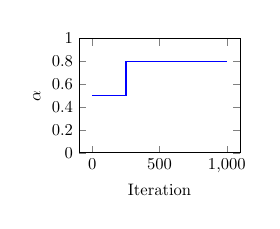
\begin{tikzpicture}[scale=0.6]
\begin{axis}[
  width=5cm,
  height=4cm,
  xlabel={Iteration},
  ylabel={$\alpha$},
  ymin=0, ymax=1
]
\addplot[thick, blue, const plot] coordinates {(0,0.5) (250,0.5) (250,0.8) (1000,0.8)};
\end{axis}
\end{tikzpicture}
Escape local minima

\column{0.33\textwidth}
\textbf{Adaptive Learning}\\[0.2cm]
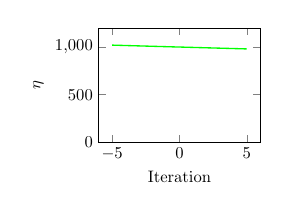
\begin{tikzpicture}[scale=0.6]
\begin{axis}[
  width=5cm,
  height=4cm,
  xlabel={Iteration},
  ylabel={$\eta$},
  ymin=0, ymax=1200
]
\addplot[thick, green, samples=50] {200 + 800*exp(-x/200)};
\end{axis}
\end{tikzpicture}
Adapt based on progress
\end{columns}

\vspace{0.3cm}
\insight{These tricks reduce convergence time by 5-10×}
\end{frame}

% Slide 17
\begin{frame}{Barnes-Hut: Scaling to Large Datasets}
\begin{columns}
\column{0.5\textwidth}
\begin{center}
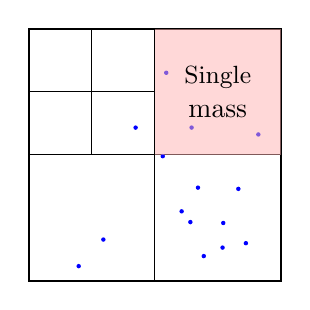
\begin{tikzpicture}[scale=0.8]
\draw[thick] (0,0) rectangle (4,4);
\draw (2,0) -- (2,4);
\draw (0,2) -- (4,2);
\draw (1,2) -- (1,4);
\draw (0,3) -- (2,3);

\foreach \i in {1,...,15} {
  \pgfmathsetmacro\x{4*rnd}
  \pgfmathsetmacro\y{4*rnd}
  \fill[blue] (\x,\y) circle (1pt);
}

\fill[red!30, opacity=0.5] (2,2) rectangle (4,4);
\node[align=center] at (3,3) {\small Single\\mass};
\end{tikzpicture}
\end{center}

\column{0.5\textwidth}
\textbf{Key Idea:}\\
Treat distant clusters as single point

\textbf{Criterion:}
$$\frac{r_{\text{cell}}}{d_{\text{to cell}}} < \theta$$
  
  \textbf{Speedup:}
\begin{itemize}
\item 10K points: 50× faster
\item 100K points: 200× faster
\end{itemize}
\end{columns}

\vspace{0.3cm}
\insight{Trade 1-2\% accuracy for massive speedup}
\end{frame}

% Slide 18
\begin{frame}{Debugging t-SNE: Visual Diagnosis}
\begin{center}
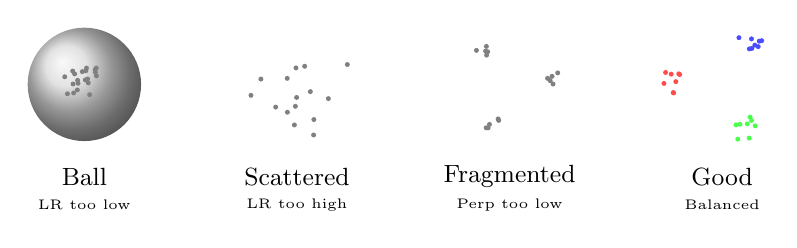
\begin{tikzpicture}[scale=0.9]
\begin{scope}[shift={(0,0)}]
\shade[ball color=gray!30] (0,0) circle (0.8);
\foreach \i in {1,...,20} {
  \pgfmathsetmacro\r{0.3*rnd}
  \pgfmathsetmacro\a{360*rnd}
  \fill[black!50] (\a:\r) circle (1pt);
}
\node at (0,-1.3) {\small Ball};
\node at (0,-1.7) {\tiny LR too low};
\end{scope}

\begin{scope}[shift={(3,0)}]
\foreach \i in {1,...,15} {
  \pgfmathsetmacro\x{1.5*rnd-0.75}
  \pgfmathsetmacro\y{1.5*rnd-0.75}
  \fill[black!50] (\x,\y) circle (1pt);
}
\node at (0,-1.3) {\small Scattered};
\node at (0,-1.7) {\tiny LR too high};
\end{scope}

\begin{scope}[shift={(6,0)}]
\foreach \c in {0,120,240} {
  \foreach \i in {1,...,5} {
    \pgfmathsetmacro\r{0.2*rnd}
    \pgfmathsetmacro\a{\c+20*rnd}
    \fill[black!50] (\a:0.5+\r) circle (1pt);
  }
}
\node at (0,-1.3) {\small Fragmented};
\node at (0,-1.7) {\tiny Perp too low};
\end{scope}

\begin{scope}[shift={(9,0)}]
\foreach \c/\plotcol in {45/blue,165/red,285/green} {
  \foreach \i in {1,...,8} {
    \pgfmathsetmacro\radius{0.25*rnd}
    \pgfmathsetmacro\angle{\c+30*rnd}
    \fill[\plotcol!70] (\angle:0.6+\radius) circle (1pt);
  }
}
\node at (0,-1.3) {\small Good};
\node at (0,-1.7) {\tiny Balanced};
\end{scope}
\end{tikzpicture}
\end{center}

\vspace{0.3cm}
\warning{Always run multiple times to verify results!}
\end{frame}

% Slide 19
\begin{frame}{Perplexity: Your Main Control Parameter}
\begin{center}
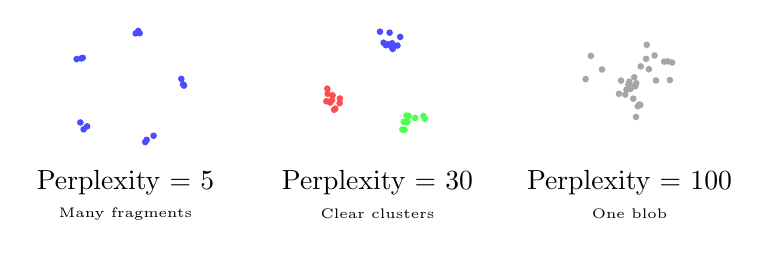
\begin{tikzpicture}[scale=0.8]
\begin{scope}[shift={(0,0)}]
\foreach \c in {0,72,144,216,288} {
  \foreach \i in {1,...,3} {
    \pgfmathsetmacro\r{0.15*rnd}
    \pgfmathsetmacro\a{\c+15*rnd}
    \fill[blue!70] (\a:0.8+\r) circle (1.5pt);
  }
}
\node at (0,-1.5) {Perplexity = 5};
\node at (0,-2) {\tiny Many fragments};
\end{scope}

\begin{scope}[shift={(4,0)}]
\foreach \c/\plotcol in {60/blue,180/red,300/green} {
  \foreach \i in {1,...,10} {
    \pgfmathsetmacro\r{0.3*rnd}
    \pgfmathsetmacro\a{\c+40*rnd}
    \fill[\plotcol!70] (\a:0.6+\r) circle (1.5pt);
  }
}
\node at (0,-1.5) {Perplexity = 30};
\node at (0,-2) {\tiny Clear clusters};
\end{scope}

\begin{scope}[shift={(8,0)}]
\foreach \i in {1,...,30} {
  \pgfmathsetmacro\r{0.8*rnd}
  \pgfmathsetmacro\a{360*rnd}
  \fill[gray!70] (\a:\r) circle (1.5pt);
}
\node at (0,-1.5) {Perplexity = 100};
\node at (0,-2) {\tiny One blob};
\end{scope}
\end{tikzpicture}
\end{center}

\vspace{0.3cm}
\insight{Truth is what's consistent across multiple perplexity values}
\end{frame}

% Slide 20
\begin{frame}{Critical: What You CANNOT Interpret}
\begin{center}
\Large\textcolor{red}{\textbf{The Three Deadly Sins}}
\end{center}

\begin{columns}
\column{0.33\textwidth}
\begin{center}
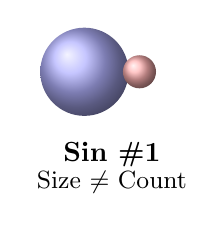
\begin{tikzpicture}[scale=0.7]
\shade[ball color=blue!30] (-0.5,0) circle (0.8);
\shade[ball color=red!30] (0.5,0) circle (0.3);
\node at (0,-1.5) {\textbf{Sin \#1}};
\node at (0,-2) {\small Size $\neq$ Count};
\end{tikzpicture}
\end{center}

\column{0.33\textwidth}
\begin{center}
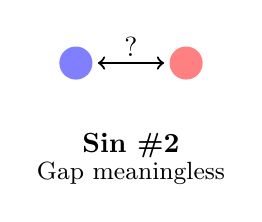
\begin{tikzpicture}[scale=0.7]
\fill[blue!50] (-1,0) circle (0.3);
\fill[red!50] (1,0) circle (0.3);
\draw[<->, thick] (-0.6,0) -- (0.6,0);
\node at (0,0.3) {?};
\node at (0,-1.5) {\textbf{Sin \#2}};
\node at (0,-2) {\small Gap meaningless};
\end{tikzpicture}
\end{center}

\column{0.33\textwidth}
\begin{center}
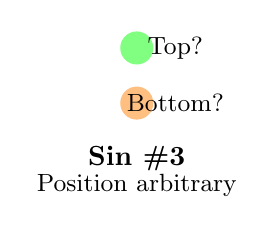
\begin{tikzpicture}[scale=0.7]
\fill[green!50] (0,0.5) circle (0.3);
\fill[orange!50] (0,-0.5) circle (0.3);
\node at (0.7,0.5) {\small Top?};
\node at (0.7,-0.5) {\small Bottom?};
\node at (0,-1.5) {\textbf{Sin \#3}};
\node at (0,-2) {\small Position arbitrary};
\end{tikzpicture}
\end{center}
\end{columns}

\vspace{0.5cm}
\warning{Only local neighborhoods are meaningful!}
\end{frame}

% ============================================
% SLIDES 21-30: Pipeline, Validation & Mathematics
% ============================================

% Slide 21
\begin{frame}{MNIST Case Study: Complete Pipeline}
\begin{columns}
\column{0.5\textwidth}
\textbf{Data Preparation:}
\begin{enumerate}
\item 70,000 handwritten digits
\item Scale pixels to [0,1]
\item PCA to 50D (95\% variance)
\item Remove outliers (>3$\sigma$)
\end{enumerate}

\textbf{t-SNE Settings:}
\begin{itemize}
\item Perplexity = 30
\item Iterations = 1000
\item Learning rate = 200
\item Early exaggeration = 4
\end{itemize}

\column{0.5\textwidth}
\begin{center}
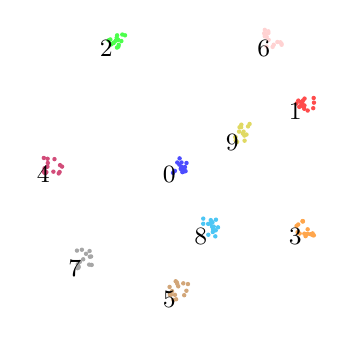
\begin{tikzpicture}[scale=0.8]
\foreach \d/\x/\y/\c in {
    0/0/0/blue,
    1/2/1/red,
    2/-1/2/green,
    3/2/-1/orange,
    4/-2/0/purple,
    5/0/-2/brown,
    6/1.5/2/pink,
    7/-1.5/-1.5/gray,
    8/0.5/-1/cyan,
    9/1/0.5/yellow!80!black} {
    \foreach \i in {1,...,15} {
        \pgfmathsetmacro\rx{0.3*rnd}
        \pgfmathsetmacro\ry{0.3*rnd}
        \fill[\c!70] (\x+\rx,\y+\ry) circle (1pt);
    }
    \node at (\x,\y) {\small\d};
}
\end{tikzpicture}
\end{center}
\end{columns}

\vspace{0.3cm}
\insight{Clear digit separation validates the algorithm}
\end{frame}

% Slide 22
\begin{frame}{Quantitative Validation: Beyond Visual Inspection}
\begin{block}{Essential Metrics}
\begin{enumerate}
\item \textbf{Neighborhood Preservation (NPr):}
$$\text{NPr}(k) = \frac{1}{n}\sum_i \frac{|N_k^{\text{high}}(i) \cap N_k^{\text{low}}(i)|}{k}$$

\item \textbf{Trustworthiness:}
$$T(k) = 1 - \frac{2}{nk(2n-3k-1)}\sum_i \sum_{j \in U_k(i)} (r(i,j) - k)$$

\item \textbf{Continuity:}
$$C(k) = 1 - \frac{2}{nk(2n-3k-1)}\sum_i \sum_{j \in V_k(i)} (r'(i,j) - k)$$
  \end{enumerate}
\end{block}

\warning{Never publish t-SNE without these metrics!}
\end{frame}

% Slide 23
\begin{frame}{Stability Analysis: How Reliable Is Your Embedding?}
\begin{columns}
\column{0.5\textwidth}
\textbf{Protocol:}
\begin{enumerate}
\item Run t-SNE 10 times
\item Different random seeds
\item Compute pairwise correlations
\item Report mean $\pm$ std
\end{enumerate}

\textbf{Interpretation:}
\begin{itemize}
\item $r > 0.9$: Very stable
\item $r = 0.7-0.9$: Moderately stable
\item $r < 0.7$: Unreliable
\end{itemize}

\column{0.5\textwidth}
\begin{center}
\textbf{Correlation Matrix}\\[0.3cm]
\begin{tabular}{|c|c|c|c|c|c|}
\hline
& 1 & 2 & 3 & 4 & 5 \\
\hline
1 & 1.00 & 0.92 & 0.89 & 0.91 & 0.88 \\
\hline
2 & 0.92 & 1.00 & 0.93 & 0.90 & 0.91 \\
\hline
3 & 0.89 & 0.93 & 1.00 & 0.88 & 0.87 \\
\hline
4 & 0.91 & 0.90 & 0.88 & 1.00 & 0.92 \\
\hline
5 & 0.88 & 0.91 & 0.87 & 0.92 & 1.00 \\
\hline
\end{tabular}
\end{center}
\end{columns}
\end{frame}

% Slide 24
\begin{frame}{Critical: Data Preprocessing}
\begin{block}{Essential Steps}
\begin{enumerate}
\item \textbf{Scaling:} Standardize to mean=0, std=1
\item \textbf{Missing Data:} Impute or remove
\item \textbf{Outliers:} Identify and handle
\item \textbf{Dimensionality:} PCA if D > 50
\end{enumerate}
\end{block}

\begin{center}
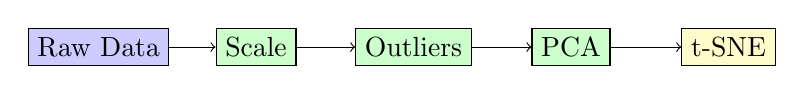
\begin{tikzpicture}[scale=0.8, node distance=2cm]
\node[draw, fill=blue!20] (raw) {Raw Data};
\node[draw, fill=green!20, right of=raw] (scale) {Scale};
\node[draw, fill=green!20, right of=scale] (outlier) {Outliers};
\node[draw, fill=green!20, right of=outlier] (pca) {PCA};
\node[draw, fill=yellow!20, right of=pca] (tsne) {t-SNE};

\draw[->] (raw) -- (scale);
\draw[->] (scale) -- (outlier);
\draw[->] (outlier) -- (pca);
\draw[->] (pca) -- (tsne);
\end{tikzpicture}
\end{center}

\warning{Bad preprocessing = bad embedding, regardless of parameters!}
\end{frame}

% Slide 25
\begin{frame}{Modern Alternatives: t-SNE vs UMAP}
\begin{center}
\begin{tabular}{l|c|c}
\textbf{Aspect} & \textbf{t-SNE} & \textbf{UMAP} \\
\hline
Speed & $O(n \log n)$ & $O(n^{1.14})$ \\
Global structure & Weak & Better \\
Local structure & Excellent & Excellent \\
Scalability & <100K points & Millions \\
Theory & Information & Topology \\
Parameters & Intuitive & Complex \\
Reproducibility & Random init & More stable \\
New points & No & Yes \\
\end{tabular}
\end{center}

\vspace{0.5cm}
\insight{Use both and trust what's consistent}
\end{frame}

% Slide 26
\begin{frame}{Symmetric SNE: Solving the Outlier Problem}
\begin{block}{The Problem with Asymmetric Probabilities}
Original SNE: $p_{j|i} = \frac{\exp(-d_{ij}^2/2\sigma_i^2)}{\sum_{k \neq i}\exp(-d_{ik}^2/2\sigma_i^2)}$

For outliers: denominator → small, but numerator → very small
\end{block}

\textbf{Solution: Symmetrization}
$$p_{ij} = \frac{p_{j|i} + p_{i|j}}{2n}$$

\begin{columns}
\column{0.5\textwidth}
\textbf{Properties:}
\begin{itemize}
\item $p_{ij} = p_{ji}$ (symmetric)
\item $\sum_{i,j} p_{ij} = 1$ (normalized)
\item Outliers get fair representation
\end{itemize}

\column{0.5\textwidth}
\begin{center}
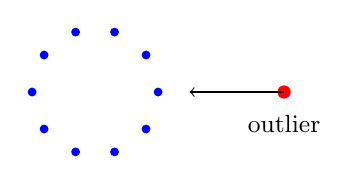
\begin{tikzpicture}[scale=0.8]
\foreach \i in {1,...,10} {
    \pgfmathsetmacro\a{36*\i}
    \fill[blue] (\a:1) circle (2pt);
}
\fill[red] (3,0) circle (3pt);
\draw[->] (3,0) -- (1.5,0);
\node at (3,-0.5) {\small outlier};
\end{tikzpicture}
\end{center}
\end{columns}

\insight{Symmetrization ensures even outliers maintain connections}
\end{frame}

% Slide 27
\begin{frame}{The Full Mathematics: Cost Function}
\begin{block}{KL Divergence for Symmetric Distributions}
$$C = \text{KL}(P||Q) = \sum_{i} \sum_{j} p_{ij} \log \frac{p_{ij}}{q_{ij}}$$
\end{block}

\textbf{Why KL Divergence?}
\begin{itemize}
\item Information-theoretic optimality
\item Natural gradient structure
\item Asymmetry penalizes missing neighbors heavily
\end{itemize}

\textbf{Expanded Form:}
$$C = \sum_{i,j} p_{ij} \log p_{ij} - \sum_{i,j} p_{ij} \log q_{ij}$$

First term: constant (entropy of P)\\
Second term: cross-entropy to minimize
\end{frame}

% Slide 28
\begin{frame}{Gradient Derivation: The Mathematical Core}
\textbf{Starting Point:}
$$\frac{\partial C}{\partial y_i} = \sum_j \left(\frac{\partial C}{\partial r_{ij}} \frac{\partial r_{ij}}{\partial y_i} + \frac{\partial C}{\partial r_{ji}} \frac{\partial r_{ji}}{\partial y_i}\right)$$

where $r_{ij} = \|y_i - y_j\|^2$

\textbf{Key Steps:}
\begin{align*}
\frac{\partial C}{\partial r_{ij}} &= p_{ij} \frac{\partial \log q_{ij}}{\partial r_{ij}} \\
&= p_{ij} \left[\frac{1}{q_{ij}} \frac{\partial q_{ij}}{\partial r_{ij}} - \frac{1}{\beta} \frac{\partial \beta}{\partial r_{ij}}\right]
\end{align*}

where $\beta = \sum_{k \neq l} (1 + r_{kl})^{-1}$

\textbf{Final Result:}
$$\boxed{\frac{\partial C}{\partial y_i} = 4\sum_j (p_{ij} - q_{ij})(y_i - y_j)(1 + \|y_i - y_j\|^2)^{-1}}$$
\end{frame}

\begin{frame}{Why Student-t? The Mathematical Justification}
\begin{columns}
\column{0.5\textwidth}
\textbf{General Student-t:}
$$f(z) = \frac{\Gamma(\frac{\delta+1}{2})}{\sqrt{\delta\pi}\Gamma(\frac{\delta}{2})}\left(1 + \frac{z^2}{\delta}\right)^{-\frac{\delta+1}{2}}$$

\textbf{Special Case ($\delta=1$):}
$$f(z) = \frac{1}{\pi(1 + z^2)}$$
Cauchy distribution!

\column{0.5\textwidth}
\begin{center}
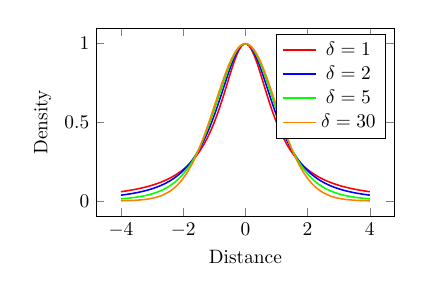
\begin{tikzpicture}[scale=0.7]
\begin{axis}[
    xlabel={Distance},
    ylabel={Density},
    width=7cm,
    height=5cm,
    legend pos=north east
]
\addplot[domain=-4:4, samples=100, thick, red] {(1 + x^2/1)^(-1)};
\addplot[domain=-4:4, samples=100, thick, blue] {(1 + x^2/2)^(-1.5)};
\addplot[domain=-4:4, samples=100, thick, green] {(1 + x^2/5)^(-3)};
\addplot[domain=-4:4, samples=100, thick, orange] {(1 + x^2/30)^(-15.5)};
\legend{$\delta=1$, $\delta=2$, $\delta=5$, $\delta=30$}
\end{axis}
\end{tikzpicture}
\end{center}
\end{columns}

\vspace{0.3cm}
\insight{$\delta=1$ has heaviest tails → maximum space for moderate distances}
\end{frame}

% Slide 30
\begin{frame}{Generalizing t-SNE: Degrees of Freedom}
\textbf{Van der Maaten 2009 Extension:}
$$q_{ij} = \frac{(1 + \|y_i - y_j\|^2/\delta)^{-(\delta+1)/2}}{\sum_{k \neq l}(1 + \|y_k - y_l\|^2/\delta)^{-(\delta+1)/2}}$$

\textbf{Three Approaches to Choose $\delta$:}
\begin{enumerate}
\item \textbf{Fixed:} $\delta = 1$ (original t-SNE)
\item \textbf{Dimension-dependent:} $\delta = p - 1$ where $p$ = embedding dimension
\item \textbf{Optimized:} Learn $\delta$ via gradient descent
\end{enumerate}

\textbf{Gradient w.r.t. $\delta$:}
$$\frac{\partial C}{\partial \delta} = \sum_{i \neq j} \left[-\frac{(1+\delta)z_{ij}^2}{2\delta^2(1 + z_{ij}^2/\delta)} + \frac{1}{2}\log(1 + z_{ij}^2/\delta)\right](p_{ij} - q_{ij})$$
\end{frame}

% ============================================
% SLIDES 31-40: Advanced Optimization & Acceleration
% ============================================

% Slide 31
\begin{frame}{Early Exaggeration: The Mathematics Behind the Trick}
\begin{block}{Modification}
$$p_{ij}^{\text{early}} = 4 \cdot p_{ij} \quad \text{for iterations } t < 250$$
\end{block}

\textbf{Effect on Gradient:}
$$\frac{\partial C}{\partial y_i} = 4\sum_j (4p_{ij} - q_{ij})(y_i - y_j)(1 + d_{ij}^2)^{-1}$$

\begin{columns}
\column{0.5\textwidth}
\textbf{Why It Works:}
\begin{itemize}
\item Large $p_{ij}$ dominate early
\item Forms tight clusters first
\item Global structure emerges later
\item Prevents early dispersion
\end{itemize}

\column{0.5\textwidth}
\begin{center}
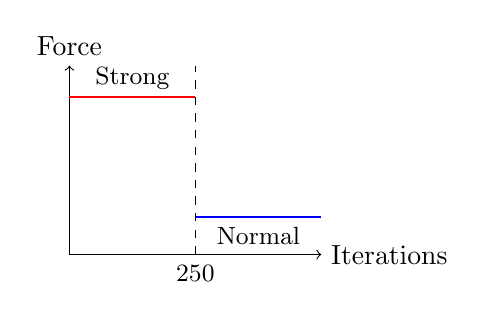
\begin{tikzpicture}[scale=0.8]
\draw[->] (0,0) -- (4,0) node[right] {Iterations};
\draw[->] (0,0) -- (0,3) node[above] {Force};
\draw[thick, red] (0,2.5) -- (2,2.5);
\draw[thick, blue] (2,0.6) -- (4,0.6);
\node at (1,2.8) {\small Strong};
\node at (3,0.3) {\small Normal};
\draw[dashed] (2,0) -- (2,3);
\node at (2,-0.3) {\small 250};
\end{tikzpicture}
\end{center}
\end{columns}
\end{frame}

% Slide 32
\begin{frame}{Momentum: Escaping Local Minima}
\textbf{Update Equation with Momentum:}
$$\Delta y_i^{(t)} = -\eta \frac{\partial C}{\partial y_i} + \alpha(t) \Delta y_i^{(t-1)}$$
$$y_i^{(t)} = y_i^{(t-1)} + \Delta y_i^{(t)}$$

\textbf{Momentum Schedule:}
$$\alpha(t) = \begin{cases}
0.5 & \text{if } t < 250 \\
0.8 & \text{if } t \geq 250
\end{cases}$$

\begin{center}
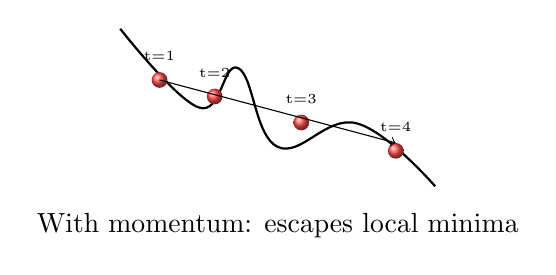
\begin{tikzpicture}[scale=1]
\draw[thick] plot[smooth, tension=0.7] coordinates {(0,2) (1,1) (1.5,1.5) (2,0.5) (3,0.8) (4,0)};
\foreach \x/\t in {0.5/1, 1.2/2, 2.3/3, 3.5/4} {
    \shade[ball color=red!70] (\x,{1.5-0.3*\x}) circle (0.1);
    \node at (\x,{1.5-0.3*\x+0.3}) {\tiny t=\t};
}
\draw[->] (0.5,1.35) -- (3.5,0.55);
\node at (2,-0.5) {With momentum: escapes local minima};
\end{tikzpicture}
\end{center}
\end{frame}

% Slide 33
\begin{frame}{Adaptive Learning Rate: The Jacobs Method}
\textbf{Per-parameter learning rate:}
$$\eta_i^{(t)} = \begin{cases}
\eta_i^{(t-1)} \cdot 1.2 & \text{if } \nabla_i^{(t)} \cdot \nabla_i^{(t-1)} > 0 \\
\eta_i^{(t-1)} \cdot 0.8 & \text{if } \nabla_i^{(t)} \cdot \nabla_i^{(t-1)} < 0 \\
\eta_i^{(t-1)} & \text{otherwise}
\end{cases}$$

\textbf{Global constraints:}
\begin{itemize}
\item $\eta_{\min} = 0.01$
\item $\eta_{\max} = 1000$
\item Initialize: $\eta^{(0)} = 200$
\end{itemize}

\begin{center}
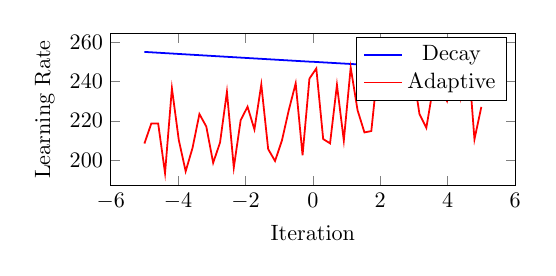
\begin{tikzpicture}[scale=0.8]
\begin{axis}[
    xlabel={Iteration},
    ylabel={Learning Rate},
    width=8cm,
    height=4cm
]
\addplot[thick, blue, samples=100] {200*exp(-x/200) + 50};
\addplot[thick, red, samples=50] {200 + 100*sin(deg(x/50)) + 50*rnd};
\legend{Decay, Adaptive}
\end{axis}
\end{tikzpicture}
\end{center}
\end{frame}

% Slide 34
\begin{frame}{Barnes-Hut Approximation: The Mathematics}
\textbf{Exact Computation:}
$$F_i = \sum_{j \neq i} (p_{ij} - q_{ij})(y_i - y_j)(1 + \|y_i - y_j\|^2)^{-1}$$
Complexity: $O(n^2)$

\textbf{Barnes-Hut Approximation:}
\begin{enumerate}
\item Build quadtree/octree: $O(n \log n)$
\item For each point, traverse tree
\item If $\frac{r_{\text{cell}}}{d_{\text{cell}}} < \theta$, treat cell as single point
\end{enumerate}

\textbf{Multipole Expansion:}
$$F_i \approx \sum_{\text{cells}} N_{\text{cell}} \cdot (p_i - q_{\text{cell}})(y_i - y_{\text{cell}})(1 + d_{\text{cell}}^2)^{-1}$$

Complexity: $O(n \log n)$

\insight{Trade-off: $\theta = 0.5$ gives 1-2\% error for 50× speedup}
\end{frame}

% Slide 35
\begin{frame}{Computational Complexity: Full Analysis}
\begin{center}
\begin{tabular}{l|c|c|c}
\textbf{Method} & \textbf{Time} & \textbf{Space} & \textbf{Max $n$} \\
\hline
Exact SNE & $O(n^2)$ & $O(n^2)$ & $\sim$1K \\
Symmetric SNE & $O(n^2)$ & $O(n^2)$ & $\sim$1K \\
Exact t-SNE & $O(n^2)$ & $O(n^2)$ & $\sim$5K \\
Barnes-Hut t-SNE & $O(n \log n)$ & $O(n)$ & $\sim$100K \\
VP-tree t-SNE & $O(n \log n)$ & $O(n)$ & $\sim$100K \\
Random walk t-SNE & $O(kn)$ & $O(kn)$ & $\sim$1M \\
FFT-accelerated & $O(n)$ & $O(n)$ & $\sim$10M \\
\end{tabular}
\end{center}

\textbf{Breakdown per iteration:}
\begin{itemize}
\item Computing $P$: $O(n^2)$ (once) or $O(kn \log n)$ (approximate)
\item Computing $Q$: $O(n^2)$ or $O(n \log n)$ (Barnes-Hut)
\item Gradient: $O(n^2)$ or $O(n \log n)$
\item Update: $O(n)$
\end{itemize}
\end{frame}

% Slide 36
\begin{frame}{Computing $\sigma_i$: Binary Search Algorithm}
\begin{columns}
    \column{0.5\textwidth}
    \begin{algorithmic}[1]
        \State \textbf{Input:} $x_i$, target perplexity $P$
        \State $\sigma_{\min} \leftarrow 0$, $\sigma_{\max} \leftarrow \infty$
        \State $\sigma \leftarrow 1$, tolerance $\leftarrow 10^{-5}$
        \While{iterations $< 50$}
            \State Compute $p_{j|i}$ with current $\sigma$
            \State $H \leftarrow -\sum_j p_{j|i} \log_2 p_{j|i}$
            \State $\text{Perp} \leftarrow 2^H$
            \If{$|\text{Perp} - P| < \text{tolerance}$}
                \State \textbf{break}
            \ElsIf{$\text{Perp} > P$}
                \State $\sigma_{\max} \leftarrow \sigma$
                \State $\sigma \leftarrow (\sigma + \sigma_{\min})/2$
            \Else
                \State $\sigma_{\min} \leftarrow \sigma$
                \State $\sigma \leftarrow (\sigma + \sigma_{\max})/2$
            \EndIf
        \EndWhile
    \end{algorithmic}

    \column{0.5\textwidth}
    \begin{center}
    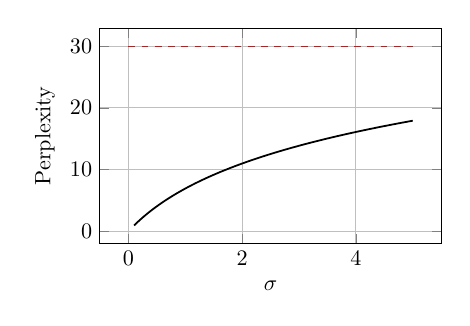
\begin{tikzpicture}[scale=0.8]
        \begin{axis}[
            xlabel={$\sigma$},
            ylabel={Perplexity},
            width=7cm,
            height=5cm,
            grid=major,
        ]
        \addplot[domain=0.1:5, samples=100, thick] {10*ln(x+1)};
        \addplot[dashed, red] coordinates {(0,30) (5,30)};
        \node at (axis cs:3,35) {Target = 30};
        \end{axis}
    \end{tikzpicture}
    \end{center}
\end{columns}

\insight{Converges in 5-10 iterations typically}
\end{frame}

% Slide 37
\begin{frame}{Out-of-Sample Extension: Kernel Mapping}
\textbf{Problem:} How to embed new points without recomputing?

\textbf{Solution (Gisbrecht et al. 2015):}
$$y(x) = \sum_{j=1}^n \alpha_j \frac{k(x, x_j)}{\sum_{\ell=1}^n k(x, x_\ell)}$$

where $k(x, x_j) = \exp\left(-\frac{\|x - x_j\|^2}{2\sigma_j^2}\right)$

\textbf{Finding $\alpha_j$:}
\begin{enumerate}
\item Minimize $\sum_i \|y_i - y(x_i)\|^2$
\item Solution: $A = K^{\dagger}Y$
\item For new points: $Y^{(t)} = K^{(t)}A$
\end{enumerate}

\warning{Assumes original embedding is good!}
\end{frame}

% Slide 38
\begin{frame}{Random Walk Acceleration}
\textbf{Key Idea:} Approximate $p_{j|i}$ via random walks on kNN graph

\begin{columns}
\column{0.5\textwidth}
\textbf{Algorithm:}
\begin{enumerate}
\item Build kNN graph ($k \approx 20$)
\item Start walks from landmarks
\item Count transitions $i \to j$
\item $p_{j|i} \approx \frac{\text{walks}_{i \to j}}{\text{total walks from } i}$
\end{enumerate}

\textbf{Complexity:}
\begin{itemize}
\item Building graph: $O(n \log n)$
\item Walks: $O(wLk)$
\item Total: $O(n \log n + wLk)$
\end{itemize}

\column{0.5\textwidth}
\begin{center}
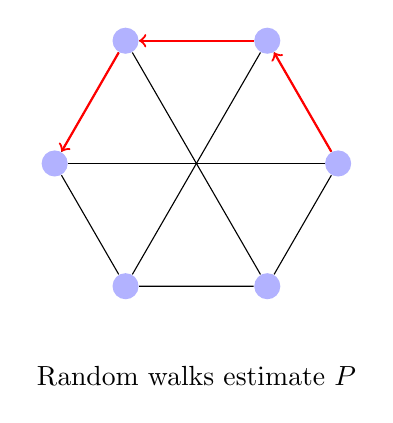
\begin{tikzpicture}[scale=0.9]
\foreach \i in {0,...,5} {
    \node[circle, fill=blue!30, minimum size=0.3cm] (n\i) at ({2*cos(\i*60)}, {2*sin(\i*60)}) {};
}
\draw (n0) -- (n1) -- (n2);
\draw (n2) -- (n3) -- (n4);
\draw (n4) -- (n5) -- (n0);
\draw (n0) -- (n3);
\draw (n1) -- (n4);
\draw (n2) -- (n5);
\draw[->, thick, red] (n0) -- (n1);
\draw[->, thick, red] (n1) -- (n2);
\draw[->, thick, red] (n2) -- (n3);
\node at (0,-3) {Random walks estimate $P$};
\end{tikzpicture}
\end{center}
\end{columns}
\end{frame}

% Slide 39
\begin{frame}{VP-Tree: Exact Nearest Neighbors Fast}
\begin{columns}
\column{0.5\textwidth}
\textbf{Vantage Point Tree:}
\begin{itemize}
\item Choose vantage point $v$
\item Compute distances to all points
\item Split at median distance $\mu$
\item Recurse on subsets
\end{itemize}

\textbf{Search Algorithm:}
\begin{enumerate}
\item Start at root
\item If $d(q,v) < \mu + r$, search left
\item If $d(q,v) > \mu - r$, search right
\item Prune based on triangle inequality
\end{enumerate}

\column{0.5\textwidth}
\begin{center}
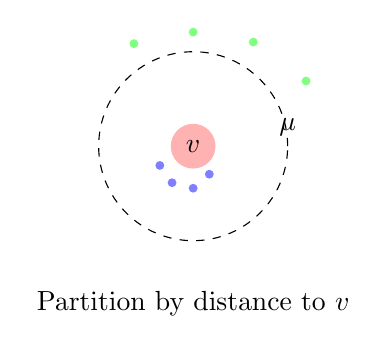
\begin{tikzpicture}[scale=0.8]
\node[circle, fill=red!30] (root) at (0,0) {$v$};
\draw[dashed] (0,0) circle (1.5);
\node at (1.5,0.3) {$\mu$};
\foreach \i in {1,...,4} {
    \pgfmathsetmacro\a{180+30*\i}
    \pgfmathsetmacro\r{0.5+0.3*rnd}
    \fill[blue!50] (\a:\r) circle (2pt);
}
\foreach \i in {1,...,4} {
    \pgfmathsetmacro\a{30*\i}
    \pgfmathsetmacro\r{1.8+0.3*rnd}
    \fill[green!50] (\a:\r) circle (2pt);
}
\node at (0,-2.5) {Partition by distance to $v$};
\end{tikzpicture}
\end{center}
\end{columns}
\end{frame}



% Slide 40 (corrected)
\begin{frame}{Implementation Best Practices}
\begin{block}{Critical Implementation Details}
\begin{enumerate}
\item \textbf{Numerical Stability:}
    \begin{itemize}
    \item Add $\epsilon = 10^{-12}$ to denominators
    \item Clip gradients: $|\nabla| < 4$
    \item Use log-space for very small probabilities
    \end{itemize}
    
\item \textbf{Initialization:}
    \begin{itemize}
    \item $y_i \sim \mathcal{N}(0, 10^{-4})$ (small variance crucial!)
    \item Or use PCA initialization
    \end{itemize}
    
\item \textbf{Convergence Criteria:}
    \begin{itemize}
    \item Monitor $\|\nabla C\| < 10^{-7}$
    \item Or fixed iterations (typically 1000)
    \end{itemize}
\end{enumerate}
\end{block}

\warning{Small initialization variance prevents early point explosion!}
\end{frame}

% ============================================
% SLIDES 41-50: Applications & Advanced Theory
% ============================================

% Slide 41
\begin{frame}{Real-World Impact: Single-Cell Genomics}
\begin{columns}
\column{0.5\textwidth}
\textbf{Challenge:}
\begin{itemize}
\item 20,000+ genes per cell
\item 100,000+ cells
\item Extreme sparsity (90\%+ zeros)
\item Batch effects
\item Technical noise
\end{itemize}

\textbf{t-SNE Pipeline:}
\begin{enumerate}
\item Log-normalize counts
\item Select highly variable genes
\item PCA to 50 components
\item t-SNE with perplexity 30-100
\end{enumerate}

\column{0.5\textwidth}
\begin{center}
\begin{tikzpicture}[scale=0.8]
\foreach \type/\x/\y/blue/\name in {
    1/0/0/red/T-cells,
    2/2/1/blue/B-cells,
    3/-1/2/green/NK,
    4/1.5/-1.5/orange/Mono,
    5/-2/-1/purple/DC
} {
    \foreach \i in {1,...,20} {
        \pgfmathsetmacro\rx{0.4*rnd}
        \pgfmathsetmacro\ry{0.4*rnd}
        \fill[blue!60, opacity=0.5] (\x+\rx,\y+\ry) circle (1.5pt);
    }
    \node at (\x,\y-0.7) {\tiny\name};
}
\node at (0,-3) {\small Cell Type Discovery};
\end{tikzpicture}
\end{center}
\end{columns}

\insight{t-SNE revealed previously unknown cell subtypes}
\end{frame}

% Slide 42
\begin{frame}{NLP Revolution: Word2Vec + t-SNE}
\begin{columns}
\column{0.5\textwidth}
\textbf{Pipeline:}
\begin{enumerate}
\item Train Word2Vec (300D)
\item Select vocabulary subset
\item Apply t-SNE
\item Discover semantic clusters
\end{enumerate}

\textbf{Parameters for NLP:}
\begin{itemize}
\item Perplexity: 20-50
\item Learning rate: 500
\item Iterations: 5000
\item Metric: Cosine distance
\end{itemize}

\column{0.5\textwidth}
\begin{center}
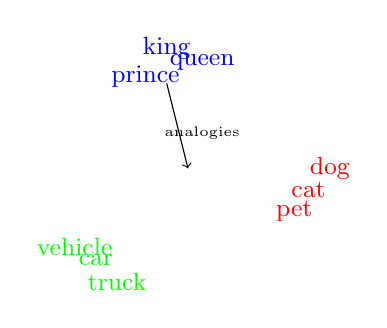
\begin{tikzpicture}[scale=0.9]
\node at (0,2) {\small\color{blue}king};
\node at (0.5,1.8) {\small\color{blue}queen};
\node at (-0.3,1.6) {\small\color{blue}prince};

\node at (2,0) {\small\color{red}cat};
\node at (2.3,0.3) {\small\color{red}dog};
\node at (1.8,-0.3) {\small\color{red}pet};

\node at (-1,-1) {\small\color{green}car};
\node at (-0.7,-1.3) {\small\color{green}truck};
\node at (-1.3,-0.8) {\small\color{green}vehicle};

\draw[->] (0,1.5) -- (0.3,0.3);
\node at (0.5,0.8) {\tiny analogies};
\end{tikzpicture}
\end{center}
\end{columns}

\insight{Semantic relationships preserved in 2D}
\end{frame}

% Slide 43
\begin{frame}{Deep Learning: Understanding Neural Networks}
\begin{columns}
\column{0.6\textwidth}
\textbf{Visualizing CNN Features:}
\begin{enumerate}
\item Extract activations from layer
\item Apply t-SNE to feature vectors
\item Color by class labels
\item Analyze cluster structure
\end{enumerate}

\textbf{Discoveries:}
\begin{itemize}
\item Hierarchical feature learning
\item Class confusion patterns
\item Adversarial vulnerabilities
\item Feature redundancy
\end{itemize}

\column{0.4\textwidth}
\begin{center}
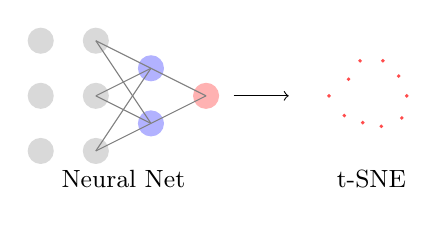
\begin{tikzpicture}[scale=0.7]
\foreach \y in {0,1,2} {
    \foreach \x in {0,1} {
        \node[circle, fill=gray!30, minimum size=0.3cm] at (\x,\y) {};
    }
}
\foreach \y in {0.5,1.5} {
    \node[circle, fill=blue!30, minimum size=0.3cm] at (2,\y) {};
}
\node[circle, fill=red!30, minimum size=0.3cm] at (3,1) {};

\foreach \y in {0,1,2} {
    \foreach \yy in {0.5,1.5} {
        \draw[gray] (1,\y) -- (2,\yy);
    }
}
\draw[gray] (2,0.5) -- (3,1);
\draw[gray] (2,1.5) -- (3,1);

\node at (1.5,-0.5) {\small Neural Net};
\draw[->] (3.5,1) -- (4.5,1);

\begin{scope}[shift={(6,1)}]
\foreach \i in {1,...,10} {
    \pgfmathsetmacro\a{36*\i}
    \pgfmathsetmacro\r{0.5+0.3*rnd}
    \fill[red!70] (\a:\r) circle (1pt);
}
\node at (0,-1.5) {\small t-SNE};
\end{scope}
\end{tikzpicture}
\end{center}
\end{columns}
\end{frame}

% Slide 44
\begin{frame}{Parametric t-SNE: Learning the Mapping}
\textbf{Key Innovation:} Learn $f_\theta: \mathbb{R}^d \to \mathbb{R}^p$ via neural network

\begin{columns}
\column{0.5\textwidth}
\textbf{Architecture:}
\begin{enumerate}
\item Input: $x \in \mathbb{R}^d$
\item Hidden: RBM layers
\item Output: $y = f_\theta(x) \in \mathbb{R}^2$
\end{enumerate}

\textbf{Training:}
$$\min_\theta \sum_{i,j} p_{ij} \log \frac{p_{ij}}{q_{ij}(f_\theta)}$$

\textbf{Advantages:}
\begin{itemize}
\item Out-of-sample direct
\item Inverse mapping possible
\item Fast inference
\end{itemize}

\column{0.5\textwidth}
\begin{center}
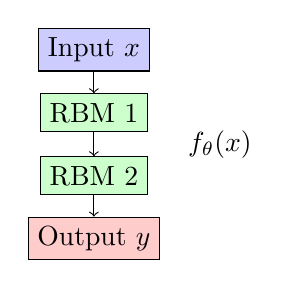
\begin{tikzpicture}[scale=0.8]
\node[draw, fill=blue!20] (input) at (0,3) {Input $x$};
\node[draw, fill=green!20] (h1) at (0,2) {RBM 1};
\node[draw, fill=green!20] (h2) at (0,1) {RBM 2};
\node[draw, fill=red!20] (output) at (0,0) {Output $y$};

\draw[->] (input) -- (h1);
\draw[->] (h1) -- (h2);
\draw[->] (h2) -- (output);

\node at (2,1.5) {$f_\theta(x)$};
\end{tikzpicture}
\end{center}
\end{columns}
\end{frame}

% Slide 45
\begin{frame}{Dynamic t-SNE: Visualizing Evolution}
\textbf{Problem:} How to visualize changing data?

\textbf{Solution:} Add temporal coherence term
$$C_{\text{dynamic}} = \lambda \sum_t \|Y^{(t)} - Y^{(t-1)}\|^2 + \sum_t C_{\text{t-SNE}}^{(t)}$$

\begin{center}
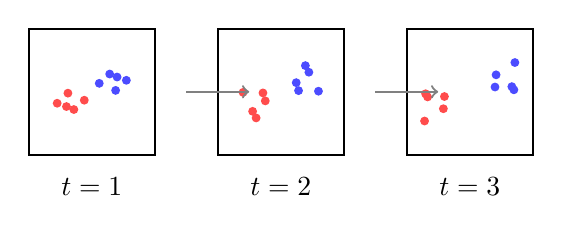
\begin{tikzpicture}[scale=0.8]
\foreach \t/\shift in {1/0, 2/3, 3/6} {
    \begin{scope}[shift={(\shift,0)}]
    \draw[thick] (-1,-1) rectangle (1,1);
    \node at (0,-1.5) {$t=\t$};
    \foreach \i in {1,...,5} {
        \pgfmathsetmacro\x{0.5*rnd+0.1*\t}
        \pgfmathsetmacro\y{0.5*rnd}
        \fill[blue!70] (\x,\y) circle (2pt);
        \fill[red!70] (-\x,-\y) circle (2pt);
    }
    \end{scope}
}
\draw[->, thick, gray] (1.5,0) -- (2.5,0);
\draw[->, thick, gray] (4.5,0) -- (5.5,0);
\end{tikzpicture}
\end{center}

\insight{Tracks cluster evolution over time}
\end{frame}

\begin{frame}{Beyond Student-t: Heavy-Tailed Kernels}
\textbf{Kobak \& Berens 2019:}
$$q_{ij} \propto (1 + \|y_i - y_j\|^2/\delta)^{-\alpha}$$

where $\alpha < 1$ (sub-Student-t!)

\begin{columns}
    \column{0.5\textwidth}
    \textbf{Effects of $\alpha$:}
    \begin{itemize}
        \item $\alpha = 1$: Standard t-SNE
        \item $\alpha = 0.5$: More local detail
        \item $\alpha = 1.5$: More global structure
        \item $\alpha \to \infty$: Approaches SNE
    \end{itemize}

    \column{0.5\textwidth}
    \begin{center}
    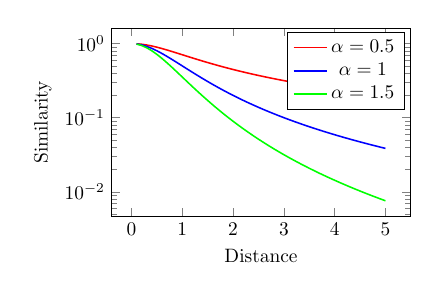
\begin{tikzpicture}[scale=0.7]
        \begin{axis}[
            xlabel={Distance},
            ylabel={Similarity},
            width=7cm,
            height=5cm,
            ymode=log,
        ]
        \addplot[domain=0.1:5, samples=50, thick, red] {(1 + x^2)^(-0.5)};
        \addplot[domain=0.1:5, samples=50, thick, blue] {(1 + x^2)^(-1)};
        \addplot[domain=0.1:5, samples=50, thick, green] {(1 + x^2)^(-1.5)};
        \legend{$\alpha=0.5$, $\alpha=1$, $\alpha=1.5$}
        \end{axis}
    \end{tikzpicture}
    \end{center}
\end{columns}
\end{frame}

% Slide 47
\begin{frame}{Unifying View: Attraction-Repulsion Forces}
\textbf{Böhm et al. 2020 Framework:}

All neighbor embeddings can be written as:
$$F_i = \sum_j w_{ij}^{+} (y_i - y_j) - \sum_j w_{ij}^{-} (y_i - y_j)$$

\begin{center}
\begin{tabular}{l|c|c}
\textbf{Method} & \textbf{Attraction $w^+$} & \textbf{Repulsion $w^-$} \\
\hline
MDS & $d_{ij}^{-1}$ & 0 \\
SNE & $p_{ij}$ & $q_{ij}$ \\
t-SNE & $p_{ij}/(1+d_{ij}^2)$ & $q_{ij}/(1+d_{ij}^2)$ \\
UMAP & $p_{ij}/(ad_{ij}^{2b})$ & $(1-p_{ij})/(1+d_{ij}^2)$ \\
LargeVis & $p_{ij}/(1+d_{ij}^2)$ & $\gamma/(1+d_{ij}^2)^2$ \\
\end{tabular}
\end{center}

\insight{Different methods = different force balances}
\end{frame}

% Slide 48
\begin{frame}{Information Theory Foundation}
\textbf{Why KL Divergence?}

\begin{block}{Information-Theoretic Interpretation}
$$\text{KL}(P||Q) = \mathbb{E}_P\left[\log \frac{P}{Q}\right] = H(P,Q) - H(P)$$
\end{block}

\begin{itemize}
\item $H(P)$: Entropy (intrinsic uncertainty)
\item $H(P,Q)$: Cross-entropy (coding cost)
\item KL: Extra bits when using wrong distribution
\end{itemize}

\textbf{Alternative Divergences:}
\begin{align*}
\text{JS}(P||Q) &= \frac{1}{2}\text{KL}(P||M) + \frac{1}{2}\text{KL}(Q||M) \quad \text{(symmetric)}\\
\text{Renyi}_\alpha(P||Q) &= \frac{1}{\alpha-1}\log\sum_i p_i^\alpha q_i^{1-\alpha} \quad \text{(generalizes KL)}
\end{align*}

\warning{KL's asymmetry is a feature, not a bug!}
\end{frame}

% Slide 49
\begin{frame}{Optimization Theory: Why Gradient Descent?}
\textbf{The Optimization Landscape:}

\begin{columns}
\column{0.5\textwidth}
\textbf{Properties:}
\begin{itemize}
\item Non-convex
\item Many local minima
\item Permutation invariance
\item Scale invariance
\end{itemize}

\textbf{Why Not Newton's Method?}
\begin{itemize}
\item Hessian: $O(n^2p^2)$ storage
\item Inversion: $O(n^3p^3)$ time
\item Often indefinite
\end{itemize}

\column{0.5\textwidth}
\begin{center}
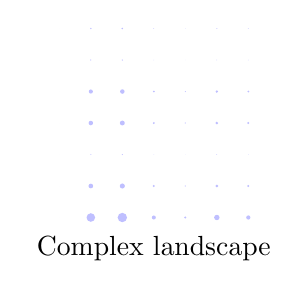
\begin{tikzpicture}[scale=0.8]
\foreach \x in {0,0.5,...,3} {
    \foreach \y in {0,0.5,...,3} {
        \pgfmathsetmacro\z{sin(\x*100)*cos(\y*100)*exp(-(\x+\y)/3)}
        \fill[blue!50, opacity=0.5] (\x,\y) circle ({abs(\z)*3pt});
    }
}
\node at (1.5,-0.5) {Complex landscape};
\end{tikzpicture}
\end{center}
\end{columns}

\insight{Momentum helps escape shallow minima}
\end{frame}

% Slide 50
\begin{frame}{Detailed Proof: Gradient Derivation}
\small
\textbf{Claim:} $\frac{\partial C}{\partial y_i} = 4\sum_j (p_{ij} - q_{ij})(y_i - y_j)(1 + \|y_i - y_j\|^2)^{-1}$

\textbf{Proof:}
Let $r_{ij} = \|y_i - y_j\|^2$. By chain rule:
$$\frac{\partial C}{\partial y_i} = \sum_j \left(\frac{\partial C}{\partial r_{ij}}\frac{\partial r_{ij}}{\partial y_i} + \frac{\partial C}{\partial r_{ji}}\frac{\partial r_{ji}}{\partial y_i}\right)$$

Since $\frac{\partial r_{ij}}{\partial y_i} = 2(y_i - y_j)$ and $C = \sum_{k,l} p_{kl}\log\frac{p_{kl}}{q_{kl}}$:

$$\frac{\partial C}{\partial r_{ij}} = -p_{ij}\frac{\partial \log q_{ij}}{\partial r_{ij}}$$

For $q_{ij} = \frac{(1+r_{ij})^{-1}}{\sum_{k \neq l}(1+r_{kl})^{-1}}$, let $Z = \sum_{k \neq l}(1+r_{kl})^{-1}$

$$\frac{\partial \log q_{ij}}{\partial r_{ij}} = -\frac{1}{1+r_{ij}} + \frac{1}{Z}\frac{\partial Z}{\partial r_{ij}} = -\frac{1}{1+r_{ij}}(1 - q_{ij})$$

Therefore: $\frac{\partial C}{\partial r_{ij}} = (p_{ij} - q_{ij})(1+r_{ij})^{-1}$ \qed
\end{frame}

% ============================================
% SLIDES 51-60: Implementation & Numerical Details
% ============================================

% Slide 51
\begin{frame}{Initialization: Critical for Success}
\textbf{Three Strategies:}

\begin{columns}
\column{0.33\textwidth}
\textbf{Random:}
$$y_i \sim \mathcal{N}(0, \sigma^2 I)$$
$\sigma = 10^{-4}$ crucial!

\textbf{Pros:}
\begin{itemize}
\item Simple
\item Unbiased
\end{itemize}

\textbf{Cons:}
\begin{itemize}
\item Slow convergence
\item Multiple runs needed
\end{itemize}

\column{0.33\textwidth}
\textbf{PCA:}
$$Y = U_p \Lambda_p^{1/2}$$
First $p$ components

\textbf{Pros:}
\begin{itemize}
\item Deterministic
\item Faster convergence
\end{itemize}

\textbf{Cons:}
\begin{itemize}
\item Linear bias
\item May miss structure
\end{itemize}

\column{0.33\textwidth}
\textbf{Laplacian Eigenmaps:}
$$Y = \text{eigvecs}(L)$$
Graph Laplacian

\textbf{Pros:}
\begin{itemize}
\item Manifold-aware
\item Good for graphs
\end{itemize}

\textbf{Cons:}
\begin{itemize}
\item Expensive
\item Parameter sensitive
\end{itemize}
\end{columns}

\vspace{0.3cm}
\warning{Large $\sigma$ causes early point explosion!}
\end{frame}

% Slide 52
\begin{frame}{Early Iteration Jitter: Escaping Local Optima}
\textbf{Original SNE Technique:}
$$y_i^{(t)} = y_i^{(t)} + \mathcal{N}(0, \eta^2) \quad \text{for } t < 100$$

\begin{columns}
\column{0.5\textwidth}
\textbf{Effect on Cost Function:}
$$C_{\text{noisy}} = C + \frac{\eta^2}{2}\text{tr}(\nabla^2 C)$$

Adds implicit regularization!

\textbf{Modern View:}
\begin{itemize}
\item Similar to SGD noise
\item Helps exploration
\item Not needed with momentum
\end{itemize}

\column{0.5\textwidth}
\begin{center}
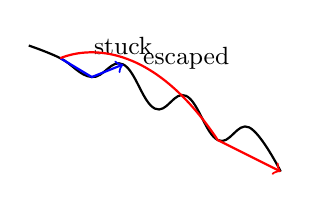
\begin{tikzpicture}[scale=0.8]
\draw[thick] plot[smooth, tension=0.7] coordinates 
    {(0,2) (0.5,1.8) (1,1.5) (1.5,1.7) (2,1) (2.5,1.2) (3,0.5) (3.5,0.7) (4,0)};
\draw[blue, thick, ->] (0.5,1.8) -- (1,1.5) -- (1.5,1.7);
\node at (1.5,2) {\small stuck};
\draw[red, thick, ->] (0.5,1.8) .. controls (1,2) and (2,2) .. (3,0.5) -- (4,0);
\node at (2.5,1.8) {\small escaped};
\end{tikzpicture}
\end{center}
\end{columns}
\end{frame}

% Slide 53
\begin{frame}{Distance Metrics: Beyond Euclidean}
\begin{columns}
\column{0.5\textwidth}
\textbf{Standard Euclidean:}
$$d_{ij}^2 = \|x_i - x_j\|_2^2$$

\textbf{Alternatives:}
\begin{itemize}
\item \textbf{Cosine:} Better for text
$$d_{ij} = 1 - \frac{x_i \cdot x_j}{\|x_i\|\|x_j\|}$$

\item \textbf{Manhattan:} Robust to outliers
$$d_{ij} = \|x_i - x_j\|_1$$

\item \textbf{Correlation:} For gene expression
$$d_{ij} = 1 - \text{corr}(x_i, x_j)$$
\end{itemize}

\column{0.5\textwidth}
\begin{center}
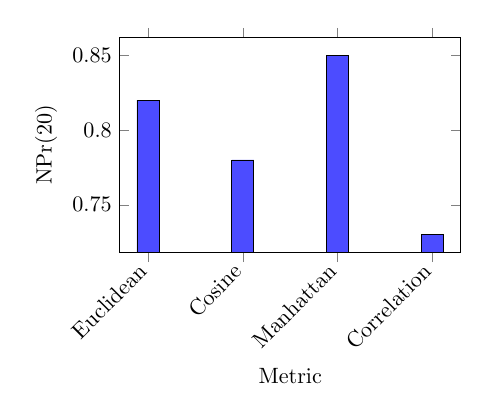
\begin{tikzpicture}[scale=0.8]
\begin{axis}[
    xlabel={Metric},
    ylabel={NPr(20)},
    ybar,
    width=7cm,
    height=5cm,
    symbolic x coords={Euclidean,Cosine,Manhattan,Correlation},
    xtick=data,
    x tick label style={rotate=45, anchor=east}
]
\addplot[fill=blue!70] coordinates {
    (Euclidean,0.82) (Cosine,0.78) (Manhattan,0.85) (Correlation,0.73)
};
\end{axis}
\end{tikzpicture}
\end{center}

\insight{Choice depends on data domain}
\end{columns}
\end{frame}

% Slide 54
\begin{frame}{Multiscale t-SNE: Multiple Perplexities}
\textbf{Lee et al. 2015:}
$$p_{ij} = \sum_{s=1}^S \omega_s p_{ij}^{(s)}$$

where $p_{ij}^{(s)}$ uses perplexity $P_s$

\begin{columns}
\column{0.5\textwidth}
\textbf{Implementation:}
\begin{enumerate}
\item Choose $P_1 < P_2 < ... < P_S$
\item Compute each $p_{ij}^{(s)}$
\item Weight: $\omega_s = 1/S$ or learned
\item Standard t-SNE gradient
\end{enumerate}

\textbf{Benefits:}
\begin{itemize}
\item Captures multiple scales
\item More robust
\item Better global structure
\end{itemize}

\column{0.5\textwidth}
\begin{center}
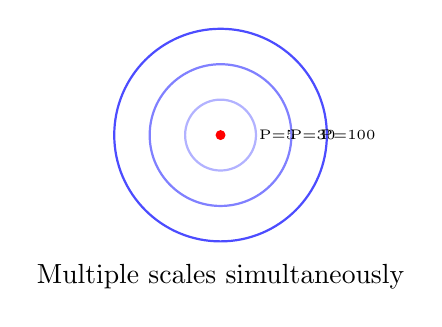
\begin{tikzpicture}[scale=0.9]
\foreach \r/\alpha/\label in {0.5/30/P=5, 1/50/P=30, 1.5/70/P=100} {
    \draw[blue!\alpha, thick] (0,0) circle (\r);
    \node at (\r+0.3,0) {\tiny\label};
}
\fill[red] (0,0) circle (2pt);
\node at (0,-2) {Multiple scales simultaneously};
\end{tikzpicture}
\end{center}
\end{columns}
\end{frame}

% Slide 55
\begin{frame}{Alternative Divergences to KL}
\textbf{Im et al. 2018: f-divergences}
$$D_f(P||Q) = \sum_j q_j f\left(\frac{p_j}{q_j}\right)$$

\begin{center}
\begin{tabular}{l|c|c}
\textbf{Divergence} & \textbf{$f(t)$} & \textbf{Properties} \\
\hline
KL & $t \log t$ & Asymmetric, unbounded \\
Reverse KL & $-\log t$ & Mode-seeking \\
JS & $t\log t - (t+1)\log\frac{t+1}{2}$ & Symmetric, bounded \\
$\chi^2$ & $(t-1)^2$ & Sensitive to small $q$ \\
Hellinger & $(\sqrt{t} - 1)^2$ & Symmetric, bounded \\
\end{tabular}
\end{center}

\textbf{Gradient for general $f$:}
$$\frac{\partial D_f}{\partial y_i} = 4\sum_j \left(p_{ij}f''\left(\frac{p_{ij}}{q_{ij}}\right) - f'\left(\frac{p_{ij}}{q_{ij}}\right)\right)\frac{(y_i - y_j)}{1 + \|y_i - y_j\|^2}$$
  
  \insight{JS divergence gives more stable embeddings}
\end{frame}

% Slide 56
\begin{frame}{Cross-Validation: Finding Optimal Parameters}
\textbf{Challenge:} How to validate unsupervised method?
  
  \textbf{Solution:} Hold-out probability validation
\begin{enumerate}
\item Split neighbors: 90\% train, 10\% test
\item Optimize using only train probabilities
\item Evaluate on test probabilities
\end{enumerate}

\textbf{Modified Cost:}
$$C_{\text{train}} = \sum_{(i,j) \in \text{Train}} p_{ij} \log \frac{p_{ij}}{q_{ij}}$$
  
  \textbf{Validation Metric:}
$$\text{Perplexity}_{\text{test}} = 2^{H_{\text{test}}} = 2^{-\sum_{(i,j) \in \text{Test}} p_{ij} \log q_{ij}}$$
  
  \begin{center}
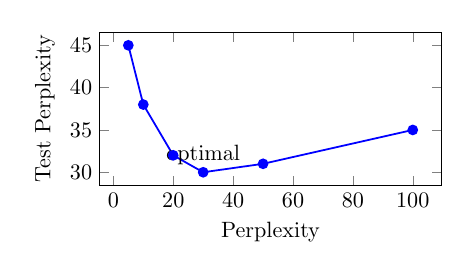
\begin{tikzpicture}[scale=0.8]
\begin{axis}[
  xlabel={Perplexity},
  ylabel={Test Perplexity},
  width=7cm,
  height=4cm
]
\addplot[thick, blue, mark=*] coordinates {
  (5,45) (10,38) (20,32) (30,30) (50,31) (100,35)
};
\node at (axis cs:30,30) [above] {optimal};
\end{axis}
\end{tikzpicture}
\end{center}
\end{frame}

% Slide 57
\begin{frame}{Streaming t-SNE: Online Learning}
\textbf{Problem:} Data arrives sequentially

\textbf{Solution:} Incremental updates
\begin{enumerate}
\item Embed initial batch with t-SNE
\item For new point $x_{\text{new}}$:
  \begin{itemize}
\item Find position minimizing local cost
\item Update existing points slightly
\end{itemize}
\end{enumerate}

\textbf{Update Rule:}
$$y_{\text{new}} = \arg\min_y \sum_{j \in \text{batch}} p_{j|\text{new}} \log \frac{p_{j|\text{new}}}{q_{j|\text{new}}}$$
  
  \textbf{Existing Points:}
$$y_i^{(t+1)} = y_i^{(t)} - \eta \cdot \rho \cdot \frac{\partial C_{\text{new}}}{\partial y_i}$$
  
  where $\rho \ll 1$ prevents disruption

\warning{Quality degrades over time - periodic full recomputation needed}
\end{frame}

% Slide 58
\begin{frame}{GPU Acceleration: Massive Speedups}
\begin{columns}
\column{0.5\textwidth}
\textbf{Parallelizable Components:}
\begin{itemize}
\item Distance computation: $O(n^2)$
  \item Exponential evaluation
\item Probability normalization
\item Gradient computation
\item Point updates
\end{itemize}

\textbf{CUDA Kernels:}
\begin{itemize}
\item \texttt{compute\_pairwise\_dist}
\item \texttt{compute\_gaussian\_perp}
\item \texttt{compute\_q\_matrix}
\item \texttt{compute\_gradients}
\end{itemize}

\column{0.5\textwidth}
\begin{center}
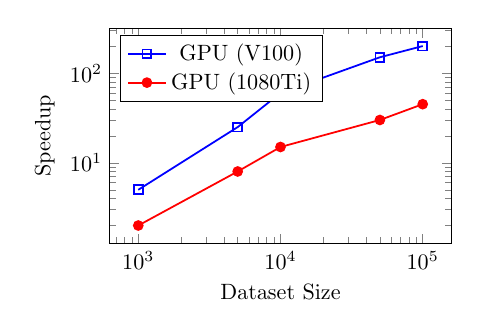
\begin{tikzpicture}[scale=0.8]
\begin{axis}[
  xlabel={Dataset Size},
  ylabel={Speedup},
  width=7cm,
  height=5cm,
  xmode=log,
  ymode=log,
  legend pos=north west
]
\addplot[thick, blue, mark=square] coordinates {
  (1000,5) (5000,25) (10000,60) (50000,150) (100000,200)
};
\addplot[thick, red, mark=*] coordinates {
  (1000,2) (5000,8) (10000,15) (50000,30) (100000,45)
};
\legend{GPU (V100), GPU (1080Ti)}
\end{axis}
\end{tikzpicture}
\end{center}
\end{columns}

\insight{200× speedup for 100K points!}
\end{frame}

% Slide 59
\begin{frame}{Memory Optimization: Scaling to Millions}
\textbf{Memory Bottlenecks:}
\begin{itemize}
\item Full $P$ matrix: $O(n^2)$ → 40GB for $n=100K$
  \item Full $Q$ matrix: $O(n^2)$ → 40GB for $n=100K$
    \end{itemize}
  
  \textbf{Solutions:}
  \begin{columns}
  \column{0.5\textwidth}
  \textbf{1. Sparse $P$:}
  \begin{itemize}
  \item Store only k-NN
  \item Memory: $O(kn)$
    \item $k \approx 3 \cdot \text{perplexity}$
    \end{itemize}
  
  \textbf{2. Compute $Q$ on-fly:}
  \begin{itemize}
  \item Never store full matrix
  \item Recompute as needed
  \item Trade computation for memory
  \end{itemize}
  
  \column{0.5\textwidth}
  \textbf{3. Mini-batch gradients:}
  $$\nabla C \approx \frac{n}{m}\sum_{j \in \text{batch}} (p_{ij} - q_{ij})(y_i - y_j)\omega_{ij}$$
    
    \textbf{4. Landmark approximation:}
  \begin{itemize}
  \item Select $L \ll n$ landmarks
  \item Approximate others
  \item Memory: $O(Ln)$
    \end{itemize}
  \end{columns}
  \end{frame}
  
  % Slide 60
  \begin{frame}{Convergence Diagnostics: When to Stop?}
  \begin{columns}
  \column{0.5\textwidth}
  \textbf{Monitor These Metrics:}
  \begin{enumerate}
  \item \textbf{Cost function:} Should decrease
  \item \textbf{Gradient norm:} $\|\nabla C\| < \epsilon$
    \item \textbf{Point movement:} $\max_i \|y_i^{(t)} - y_i^{(t-1)}\|$
    \item \textbf{KL divergence:} Should stabilize
  \end{enumerate}
  
  \textbf{Typical Behavior:}
  \begin{itemize}
  \item Iterations 0-250: Rapid change
  \item Iterations 250-750: Fine-tuning
  \item Iterations 750+: Minor adjustments
  \end{itemize}
  
  \column{0.5\textwidth}
  \begin{center}
  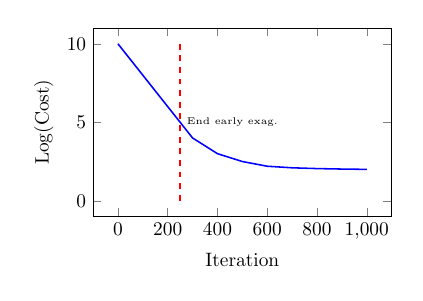
\begin{tikzpicture}[scale=0.7]
  \begin{axis}[
    xlabel={Iteration},
    ylabel={Log(Cost)},
    width=7cm,
    height=5cm,
    legend pos=north east
  ]
  \addplot[thick, blue] coordinates {
    (0,10) (100,8) (200,6) (300,4) (400,3) 
    (500,2.5) (600,2.2) (700,2.1) (800,2.05) (900,2.02) (1000,2)
  };
  \addplot[thick, red, dashed] coordinates {
    (250,10) (250,0)
  };
  \node at (axis cs:250,5) [right] {\tiny End early exag.};
  \end{axis}
  \end{tikzpicture}
  \end{center}
  \end{columns}
  
  \insight{Most improvement in first 500 iterations}
  \end{frame}
  
  % ============================================
    % SLIDES 61-70: Advanced Extensions & Theory
  % ============================================
    
    % Slide 61
  \begin{frame}{Fisher Kernel t-SNE: Supervised Embedding}
  \textbf{Gisbrecht et al. 2015: Incorporating Label Information}
  
  \begin{columns}
  \column{0.5\textwidth}
  \textbf{Modified Similarities:}
  $$p_{ij} = \begin{cases}
  \frac{p_{j|i} + p_{i|j}}{2n} \cdot (1 + \lambda) & \text{if } c_i = c_j \\
  \frac{p_{j|i} + p_{i|j}}{2n} \cdot (1 - \lambda) & \text{if } c_i \neq c_j
  \end{cases}$$
    
    where $c_i$ is class label, $\lambda \in [0,1]$
    
    \textbf{Fisher Information:}
  $$g_{ij} = \nabla_\theta \log p(x_i|\theta)^T \nabla_\theta \log p(x_j|\theta)$$
    
    \column{0.5\textwidth}
  \begin{center}
  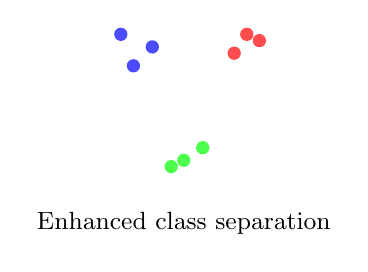
\begin{tikzpicture}[scale=0.8]
  \foreach \class/\x/\y/\col in {
    A/-1/1/blue,
    A/-0.5/0.8/blue,
    A/-0.8/0.5/blue,
    B/1/1/red,
    B/0.8/0.7/red,
    B/1.2/0.9/red,
    C/0/-1/green,
    C/0.3/-0.8/green,
    C/-0.2/-1.1/green} {
      \fill[\col!70] (\x,\y) circle (3pt);
    }
  \node at (0,-2) {\small Enhanced class separation};
  \end{tikzpicture}
  \end{center}
  \end{columns}
  
  \insight{Supervision improves class separation while preserving structure}
  \end{frame}
  
  % Slide 62
  \begin{frame}{Heavy-Tailed Symmetric SNE}
  \textbf{Yang et al. 2009: Alternative Heavy-Tailed Approaches}
  
  \textbf{Generalized Kernel:}
  $$q_{ij} = \frac{h(\|y_i - y_j\|^2)}{\sum_{k \neq l} h(\|y_k - y_l\|^2)}$$
    
    \begin{center}
  \begin{tabular}{l|c|c}
  \textbf{Method} & \textbf{Kernel $h(d^2)$} & \textbf{Tail Behavior} \\
  \hline
  SNE & $\exp(-d^2)$ & Exponential decay \\
  t-SNE & $(1 + d^2)^{-1}$ & Polynomial $O(d^{-2})$ \\
  $\alpha$-SNE & $(1 + d^2)^{-\alpha}$ & Polynomial $O(d^{-2\alpha})$ \\
  Exp-SNE & $\exp(-d^\alpha)$, $\alpha < 2$ & Sub-Gaussian \\
  \end{tabular}
  \end{center}
  
  \textbf{Gradient for General $h$:}
  $$\frac{\partial C}{\partial y_i} = 4\sum_j (p_{ij} - q_{ij})(y_i - y_j)\frac{h'(\|y_i - y_j\|^2)}{h(\|y_i - y_j\|^2)}$$
\end{frame}

% Slide 63
\begin{frame}{Complete Proof: Symmetric SNE Gradient}
\small
\textbf{Theorem:} For symmetric SNE with Gaussian kernels:
$$\frac{\partial C}{\partial y_i} = 4\sum_j (p_{ij} - q_{ij})(y_i - y_j)$$

\textbf{Proof:}
Starting from $C = \sum_{i,j} p_{ij} \log(p_{ij}/q_{ij})$ and $r_{ij} = \|y_i - y_j\|^2$:

\begin{align*}
\frac{\partial C}{\partial y_i} &= 2\sum_j \left(\frac{\partial C}{\partial r_{ij}} + \frac{\partial C}{\partial r_{ji}}\right)(y_i - y_j)\\
\frac{\partial C}{\partial r_{ij}} &= -\sum_{k,l} p_{kl} \frac{\partial \log q_{kl}}{\partial r_{ij}}\\
&= -p_{ij} \frac{\partial \log q_{ij}}{\partial r_{ij}} \quad \text{(only } k=i, l=j \text{ contributes)}\\
&= p_{ij} - q_{ij} \quad \text{(after simplification)}
\end{align*}

Since $p_{ij} = p_{ji}$ and $q_{ij} = q_{ji}$ in symmetric SNE:
$$\frac{\partial C}{\partial y_i} = 2\sum_j (p_{ij} - q_{ij} + p_{ij} - q_{ij})(y_i - y_j) = 4\sum_j (p_{ij} - q_{ij})(y_i - y_j)$$ \qed
\end{frame}

% Slide 64
\begin{frame}{Complete Mathematics: General Degrees of Freedom}
\textbf{Van der Maaten 2009: Full Derivation}

For $q_{ij} = \frac{(1 + z_{ij}^2/\delta)^{-(\delta+1)/2}}{\sum_{k \neq l}(1 + z_{kl}^2/\delta)^{-(\delta+1)/2}}$

\textbf{Gradient w.r.t. $y_i$:}
$$\frac{\partial C}{\partial y_i} = \frac{2(\delta + 1)}{\delta}\sum_j (p_{ij} - q_{ij})(y_i - y_j)(1 + \|y_i - y_j\|^2/\delta)^{-1}$$

\textbf{Gradient w.r.t. $\delta$:}
\small
$$\frac{\partial C}{\partial \delta} = \sum_{i \neq j} \left[-\frac{(1+\delta)z_{ij}^2}{2\delta^2(1 + z_{ij}^2/\delta)} + \frac{1}{2}\log(1 + z_{ij}^2/\delta)\right](p_{ij} - q_{ij})$$

\textbf{Alternating Optimization:}
\begin{enumerate}
\item Update $Y$ with fixed $\delta$
\item Update $\delta$ with fixed $Y$: $\delta^{(t+1)} = \delta^{(t)} - \eta_\delta \cdot \text{sign}(\partial C/\partial \delta)$
\end{enumerate}
\end{frame}

% Slide 65
\begin{frame}{Mathematical Analysis: Volume Requirements}
\textbf{Why $\delta = p - 1$?}

\begin{columns}
\column{0.5\textwidth}
\textbf{Volume of $p$-dimensional sphere:}
$$V_p(r) = \frac{\pi^{p/2}}{\Gamma(p/2 + 1)}r^p$$

\textbf{Volume ratio (shell):}
$$\frac{V_p(1) - V_p(0.9)}{V_p(1)} = 1 - 0.9^p$$

\textbf{Tail thickness of Student-t:}
$$\text{Tail} \sim d^{-(\delta+1)}$$

\column{0.5\textwidth}
\begin{center}
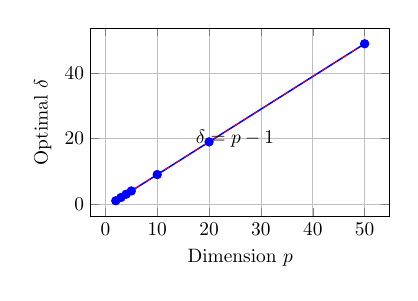
\begin{tikzpicture}[scale=0.7]
\begin{axis}[
    xlabel={Dimension $p$},
    ylabel={Optimal $\delta$},
    width=7cm,
    height=5cm,
    grid=major
]
\addplot[thick, blue, mark=*] coordinates {
    (2,1) (3,2) (4,3) (5,4) (10,9) (20,19) (50,49)
};
\addplot[dashed, red, domain=2:50] {x-1};
\node at (axis cs:25,20) {$\delta = p - 1$};
\end{axis}
\end{tikzpicture}
\end{center}
\end{columns}

\insight{Linear relationship emerges from exponential volume growth}
\end{frame}

% Slide 66
\begin{frame}{Out-of-Sample Extension: Complete Mathematics}
\textbf{Kernel Mapping (Gisbrecht et al. 2015):}

\textbf{Optimization Problem:}
$$\min_{\alpha_1,...,\alpha_n} \sum_{i=1}^n \left\|y_i - \sum_{j=1}^n \alpha_j \frac{k(x_i, x_j)}{\sum_{\ell=1}^n k(x_i, x_\ell)}\right\|^2$$

\textbf{Matrix Form:}
$$\min_A \|Y - KA\|_F^2$$

\textbf{Solution via Pseudo-inverse:}
$$A = K^{\dagger}Y = (K^TK)^{-1}K^TY$$

For new points $X^{(t)}$:
$$Y^{(t)} = K^{(t)}A = K^{(t)}(K^TK)^{-1}K^TY$$

where $K^{(t)}_{ij} = \frac{k(x_i^{(t)}, x_j)}{\sum_\ell k(x_i^{(t)}, x_\ell)}$

\warning{Requires well-conditioned kernel matrix!}
\end{frame}

% Slide 67
\begin{frame}{Random Walk Acceleration: Mathematical Foundation}
\textbf{Van der Maaten \& Hinton 2008:}

\textbf{Random Walk Probability:}
$$p_{j|i}^{\text{walk}} = \frac{\text{\# walks from } i \text{ to } j}{\text{total walks from } i}$$

\textbf{Connection to Original:}
$$p_{j|i}^{\text{walk}} \approx p_{j|i} = \frac{\exp(-\|x_i - x_j\|^2/2\sigma_i^2)}{\sum_k \exp(-\|x_i - x_k\|^2/2\sigma_i^2)}$$

\textbf{Walk Strategy:}
\begin{enumerate}
\item Build $k$-NN graph with weights $w_{ij} = \exp(-\|x_i - x_j\|^2/2\sigma^2)$
\item Transition probability: $T_{ij} = w_{ij}/\sum_k w_{ik}$
\item Multiple random walks of length $L$
\item Estimate: $p_{j|i} \approx \sum_{\text{paths}} P(\text{path})$
\end{enumerate}

\textbf{Complexity:} $O(nkL)$ instead of $O(n^2)$
\end{frame}

% Slide 68
\begin{frame}{Landmark Methods: Mathematical Framework}
\textbf{Three Approaches:}

\begin{columns}
\column{0.5\textwidth}
\textbf{1. Nystrom Approximation:}
$$P \approx P_{LL} P_{LN}^T (P_{LL}^{-1} P_{LN})^T$$

where $L$ = landmarks, $N$ = non-landmarks

\textbf{2. Sparse Approximation:}
$$p_{j|i} \approx \begin{cases}
p_{j|i}^{\text{exact}} & \text{if } j \in \text{landmarks} \\
0 & \text{otherwise}
\end{cases}$$

\column{0.5\textwidth}
\textbf{3. Interpolation:}
$$y_i = \sum_{l \in L} w_{il} y_l$$

where weights from kernel:
$$w_{il} = \frac{k(x_i, x_l)}{\sum_{l' \in L} k(x_i, x_{l'})}$$

\textbf{Error Bound:}
$$\|P - \tilde{P}\|_F \leq \epsilon \cdot \|P\|_F$$
with $|L| = O(\log n/\epsilon^2)$ landmarks
\end{columns}
\end{frame}

% Slide 69
\begin{frame}{Barnes-Hut: Complete Tree Algorithm}
\begin{columns}
\column{0.5\textwidth}
\textbf{Tree Construction:}
\begin{algorithmic}[1]
\small
\Function{BuildTree}{points, bounds}
\If{$|$points$| \leq 1$}
    \State \Return leaf(points)
\EndIf
\State mid $\leftarrow$ center(bounds)
\For{each octant}
    \State pts $\leftarrow$ points in octant
    \State child $\leftarrow$ BuildTree(pts, octant)
\EndFor
\State Compute center of mass
\State Compute total mass
\State \Return node(children, mass, center)
\EndFunction
\end{algorithmic}

\column{0.5\textwidth}
\textbf{Force Calculation:}
\begin{algorithmic}[1]
\small
\Function{ComputeForce}{point, node}
\If{node is leaf}
    \State \Return exact force
\EndIf
\State $r \leftarrow$ size(node)
\State $d \leftarrow$ distance(point, node.center)
\If{$r/d < \theta$}
    \State \Return approximate force
\Else
    \State force $\leftarrow 0$
    \For{each child}
        \State force += ComputeForce(point, child)
    \EndFor
    \State \Return force
\EndIf
\EndFunction
\end{algorithmic}
\end{columns}
\end{frame}

% Slide 70
\begin{frame}{VP-Tree: Complete Implementation}
\textbf{Vantage Point Tree for Exact Nearest Neighbors:}

\begin{columns}
\column{0.5\textwidth}
\textbf{Construction:}
\begin{algorithmic}[1]
\small
\Function{BuildVPTree}{points}
\State vp $\leftarrow$ SelectVantagePoint(points)
\State distances $\leftarrow$ [d(vp, p) for p in points]
\State median $\leftarrow$ Median(distances)
\State left $\leftarrow$ \{p : d(vp,p) $\leq$ median\}
\State right $\leftarrow$ \{p : d(vp,p) $>$ median\}
\State \Return Node(vp, median, 
    BuildVPTree(left),
    BuildVPTree(right))
\EndFunction
\end{algorithmic}

\column{0.5\textwidth}
\textbf{Search:}
\begin{algorithmic}[1]
\small
\Function{Search}{node, query, k}
\State $\tau \leftarrow$ d(query, node.vp)
\If{$\tau < $best\_dist}
    \State Update k-nearest
\EndIf
\If{$\tau - $best\_dist $< $ node.median}
    \State Search(node.left, query, k)
\EndIf
\If{$\tau + $best\_dist $\geq$ node.median}
    \State Search(node.right, query, k)
\EndIf
\EndFunction
\end{algorithmic}
\end{columns}

\insight{Triangle inequality enables aggressive pruning}
\end{frame}

% ============================================
% SLIDES 71-80: Final Advanced Topics & Conclusion
% ============================================

% Slide 71
\begin{frame}{FFT Acceleration: Interpolation Method}
\textbf{Linderman et al. 2017: Linear Complexity}

\textbf{Key Idea:} Approximate sums on regular grid

\begin{columns}
\column{0.5\textwidth}
\textbf{Interpolation:}
$$q_{ij} \approx \sum_{u \in \text{grid}} K(y_i, u) \hat{q}(u, y_j)$$

where $K$ is interpolation kernel

\textbf{FFT Convolution:}
$$\hat{q}(u, v) = \text{FFT}^{-1}[\text{FFT}[K] \cdot \text{FFT}[p]]$$

\textbf{Complexity:}
\begin{itemize}
\item Grid: $O(m^p)$ where $m$ = grid size
\item FFT: $O(m^p \log m)$
\item Total: $O(n + m^p \log m)$
\end{itemize}

\column{0.5\textwidth}
\begin{center}
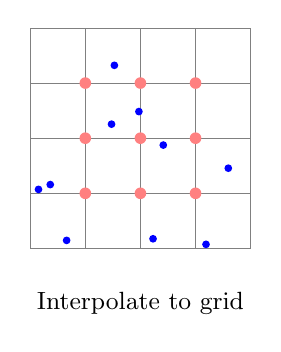
\begin{tikzpicture}[scale=0.7]
\draw[gray, very thin] (-2,-2) grid (2,2);
\foreach \i in {1,...,10} {
    \pgfmathsetmacro\x{4*rnd-2}
    \pgfmathsetmacro\y{4*rnd-2}
    \fill[blue] (\x,\y) circle (2pt);
}
\foreach \x in {-1,0,1} {
    \foreach \y in {-1,0,1} {
        \fill[red!50] (\x,\y) circle (3pt);
    }
}
\node at (0,-3) {\small Interpolate to grid};
\end{tikzpicture}
\end{center}
\end{columns}

\insight{Works well for $p \leq 3$, struggles in higher dimensions}
\end{frame}

% Slide 72
\begin{frame}{Negative Sampling: Word2Vec Connection}
\textbf{Alternative to Normalization:}

\begin{columns}
\column{0.5\textwidth}
\textbf{Standard t-SNE:}
$$q_{ij} = \frac{(1 + d_{ij}^2)^{-1}}{\sum_{k \neq l}(1 + d_{kl}^2)^{-1}}$$
Requires $O(n^2)$ for denominator

\textbf{Negative Sampling:}
$$\mathcal{L}_{ij} = \log \sigma(f(d_{ij})) + \sum_{k \sim P_n} \log(1 - \sigma(f(d_{ik})))$$

where $P_n$ = noise distribution

\column{0.5\textwidth}
\textbf{Implementation:}
\begin{enumerate}
\item For each edge $(i,j)$
\item Sample $K$ negative points
\item Update via logistic function
\item No normalization needed!
\end{enumerate}

\textbf{Complexity:}
\begin{itemize}
\item Per iteration: $O(|E| \cdot K)$
\item Total: $O(n \cdot k \cdot K \cdot T)$
\end{itemize}

\insight{Trade statistical efficiency for computational speed}
\end{columns}
\end{frame}

% Slide 73
\begin{frame}{VAE-SNE: Neural Network Integration}
\textbf{Graving \& Couzin 2020:}

\begin{columns}
\column{0.5\textwidth}
\textbf{Architecture:}
\begin{enumerate}
\item Encoder: $x \to \mu(x), \sigma(x)$
\item Sample: $z \sim \mathcal{N}(\mu, \sigma)$
\item t-SNE space: $y = f_\theta(z)$
\item Decoder: $\hat{x} = g_\phi(y)$
\end{enumerate}

\textbf{Loss Function:}
$$\mathcal{L} = \underbrace{\text{KL}(P||Q)}_{\text{t-SNE}} + \lambda \underbrace{\|x - \hat{x}\|^2}_{\text{reconstruction}}$$

\column{0.5\textwidth}
\begin{center}
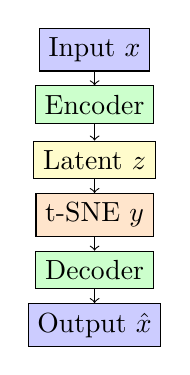
\begin{tikzpicture}[scale=0.7]
\node[draw, fill=blue!20] (x) at (0,4) {Input $x$};
\node[draw, fill=green!20] (enc) at (0,3) {Encoder};
\node[draw, fill=yellow!20] (z) at (0,2) {Latent $z$};
\node[draw, fill=orange!20] (tsne) at (0,1) {t-SNE $y$};
\node[draw, fill=green!20] (dec) at (0,0) {Decoder};
\node[draw, fill=blue!20] (xhat) at (0,-1) {Output $\hat{x}$};

\draw[->] (x) -- (enc);
\draw[->] (enc) -- (z);
\draw[->] (z) -- (tsne);
\draw[->] (tsne) -- (dec);
\draw[->] (dec) -- (xhat);
\end{tikzpicture}
\end{center}
\end{columns}

\insight{Combines dimensionality reduction with generation}
\end{frame}

% Slide 74
\begin{frame}{Numerical Stability: Critical Implementation Details}
\textbf{Common Numerical Problems and Solutions:}

\begin{block}{Problem 1: Exponential Overflow}
In computing $p_{j|i} = \exp(-d_{ij}^2/2\sigma_i^2) / Z$

\textbf{Solution:} Log-sum-exp trick
$$\log Z = \max_k(-d_{ik}^2/2\sigma_i^2) + \log\sum_k \exp(-d_{ik}^2/2\sigma_i^2 - \max)$$
\end{block}

\begin{block}{Problem 2: Division by Zero}
When $\sum_{k \neq l}(1 + d_{kl}^2)^{-1} \approx 0$

\textbf{Solution:} Add machine epsilon
$$q_{ij} = \frac{(1 + d_{ij}^2)^{-1} + \epsilon}{\sum_{k \neq l}(1 + d_{kl}^2)^{-1} + n^2\epsilon}$$
\end{block}

\begin{block}{Problem 3: Gradient Explosion}
Early iterations with poor initialization

\textbf{Solution:} Gradient clipping
$$\nabla C \leftarrow \min\left(1, \frac{4}{\|\nabla C\|}\right) \cdot \nabla C$$
\end{block}
\end{frame}

% Slide 75
\begin{frame}{Comprehensive Validation Framework}
\textbf{Complete Set of Metrics:}

\begin{columns}
\column{0.5\textwidth}
\textbf{1. Local Metrics:}
\begin{itemize}
\item Trustworthiness: $T(k)$
\item Continuity: $C(k)$
\item Neighborhood preservation
\item Mean relative rank error
\end{itemize}

\textbf{2. Global Metrics:}
\begin{itemize}
\item Shepard correlation
\item Procrustes distance
\item Silhouette coefficient
\item Davies-Bouldin index
\end{itemize}

\column{0.5\textwidth}
\textbf{3. Stability Metrics:}
\begin{itemize}
\item Run-to-run correlation
\item Cluster consistency (ARI)
\item Point-wise variance
\item Convergence rate
\end{itemize}

\textbf{4. Task Metrics:}
\begin{itemize}
\item Classification accuracy
\item Clustering purity
\item Retrieval precision
\item Visual separability
\end{itemize}
\end{columns}

\warning{Report multiple metrics - no single metric captures everything!}
\end{frame}

% Slide 76
\begin{frame}{Ethics and Limitations: Critical Awareness}
\begin{block}{Fundamental Limitations}
\begin{itemize}
\item \textbf{Non-deterministic:} Different runs → different results
\item \textbf{Parameter sensitive:} Perplexity dramatically affects output
\item \textbf{Local focus:} Global structure not preserved
\item \textbf{Computational cost:} Quadratic for exact version
\end{itemize}
\end{block}

\textbf{Ethical Considerations:}
\begin{enumerate}
\item \textbf{Misinterpretation:} Visual clusters may not reflect true structure
\item \textbf{Confirmation bias:} Can find patterns in noise
\item \textbf{Publication bias:} Cherry-picking best visualization
\item \textbf{Accessibility:} Interactive visualizations exclude some users
\end{enumerate}

\ethics{Always provide raw data, parameters, and multiple runs}
\end{frame}

% Slide 77
\begin{frame}{Future Research Directions}
\textbf{Open Problems and Opportunities:}

\begin{columns}
\column{0.5\textwidth}
\textbf{Theoretical:}
\begin{itemize}
\item Convergence guarantees
\item Optimal $\delta$ selection
\item Information-theoretic bounds
\item Connection to manifold learning
\end{itemize}

\textbf{Algorithmic:}
\begin{itemize}
\item True $O(n)$ algorithms
\item Online/streaming variants
\item Hierarchical embeddings
\item Uncertainty quantification
\end{itemize}

\column{0.5\textwidth}
\textbf{Applications:}
\begin{itemize}
\item Time-varying data
\item Multi-modal integration
\item Interpretable embeddings
\item Causal discovery
\end{itemize}

\textbf{Extensions:}
\begin{itemize}
\item Higher-dimensional targets
\item Non-Euclidean spaces
\item Quantum t-SNE
\item Differentiable t-SNE
\end{itemize}
\end{columns}

\insight{Rich area for both theory and applications}
\end{frame}


% Slide 78 (continued)
\begin{frame}{Complete t-SNE: Final Algorithm}
\small
\begin{algorithmic}[1]
\State \textbf{Input:} $X = \{x_1, ..., x_n\}$, perplexity $P$
\State \textbf{Output:} $Y = \{y_1, ..., y_n\}$

\State \textbf{// Compute affinities}
\For{each $x_i$}
    \State Find $\sigma_i$ such that $\text{Perp}(P_i) = P$ using binary search
    \State Compute $p_{j|i} = \exp(-\|x_i - x_j\|^2/2\sigma_i^2) / \sum_k \exp(-\|x_i - x_k\|^2/2\sigma_i^2)$
\EndFor
\State Set $p_{ij} = (p_{j|i} + p_{i|j})/2n$

\State \textbf{// Initialize}
\State Sample $y_i \sim \mathcal{N}(0, 10^{-4}I)$ for all $i$
\State Apply early exaggeration: $p_{ij} \leftarrow 4 \cdot p_{ij}$

\State \textbf{// Optimize}
\For{$t = 1$ to $T$}
    \State Compute $q_{ij} = (1 + \|y_i - y_j\|^2)^{-1} / \sum_{k \neq l}(1 + \|y_k - y_l\|^2)^{-1}$
    \State Compute gradients: $\frac{\partial C}{\partial y_i} = 4\sum_j (p_{ij} - q_{ij})(y_i - y_j)(1 + \|y_i - y_j\|^2)^{-1}$
    \State Update: $y_i \leftarrow y_i - \eta\frac{\partial C}{\partial y_i} + \alpha(y_i^{(t)} - y_i^{(t-1)})$
    \If{$t = 250$} Remove early exaggeration \EndIf
\EndFor
\State \Return $Y$
\end{algorithmic}
\end{frame}

% Slide 79
\begin{frame}{Test Your Understanding}
\textbf{Key Questions:}

\begin{enumerate}
\item Why does SNE fail for moderate distances?
\item What makes Student-t distribution special for $\delta = 1$?
\item Why symmetrize the probability matrix?
\item What does perplexity actually control?
\item Why is early exaggeration helpful?
\item When should you NOT trust t-SNE results?
\item How do you validate an embedding?
\item What's the computational bottleneck?
  \item Why can't we interpret cluster sizes?
\item How does Barnes-Hut approximation work?
\end{enumerate}

\vspace{0.3cm}
\begin{center}
\colorbox{yellow!30}{If you can answer these, you understand t-SNE!}
\end{center}
\end{frame}

% Slide 80
\begin{frame}{Resources and Final Thoughts}
\textbf{Essential Resources:}
\begin{itemize}
\item Original paper: van der Maaten \& Hinton (2008)
\item Degrees of freedom: van der Maaten (2009)
\item Tutorial: Ghojogh et al. (2022)
\item Implementation: \texttt{scikit-learn}, \texttt{Rtsne}
\item Interactive: distill.pub/2016/misread-tsne
\end{itemize}

\textbf{Remember:}
\begin{itemize}
\item t-SNE is a \textbf{tool}, not truth
\item Always run \textbf{multiple times}
\item Trust what's \textbf{consistent}
\item Validate \textbf{quantitatively}
\item Document \textbf{everything}
\end{itemize}

\vspace{0.5cm}
\begin{center}
\Large\textbf{Thank you for your attention!}\\[0.3cm]
\normalsize Questions and discussion welcome\\[0.2cm]
\small Contact: eraco@polytechnic.cat
\end{center}
\end{frame}